\documentclass[12pt,a4paper]{report}

% ── Core packages ──────────────────────────────────────────────────────────────
\usepackage[utf8]{inputenc}
\usepackage[T1]{fontenc}
\usepackage{lmodern}
\usepackage{microtype}          % better line breaking, prevents overfull hboxes
\usepackage{acronym}
\usepackage{amssymb}
\usepackage{amsmath}
\usepackage{amsfonts}
\usepackage{bm}
\usepackage{graphicx}
\usepackage{wrapfig}
\usepackage{float}
\usepackage{booktabs}
\usepackage{multirow}
\usepackage{multicol}
\usepackage{rotating}
\usepackage{longtable}
\usepackage{tabularx}           % auto-width columns
\usepackage{array}
\usepackage{xcolor}
\usepackage{caption}
\usepackage{ragged2e}
\usepackage{anyfontsize}
\usepackage{setspace}
\usepackage{parskip}
\usepackage{lineno}
\usepackage{comment}
\usepackage{natbib}
\usepackage[toc,page]{appendix}
\usepackage{blindtext}

% ── Geometry ───────────────────────────────────────────────────────────────────
\usepackage[left=3.5cm, right=2.0cm, top=2.5cm, bottom=2.5cm]{geometry}

% ── TikZ ───────────────────────────────────────────────────────────────────────
\usepackage{tikz}
\usetikzlibrary{shapes.geometric, arrows, positioning, fit, calc,
                decorations.pathreplacing}

% ── Listings ───────────────────────────────────────────────────────────────────
\usepackage{listings}
\lstset{
  basicstyle    = \ttfamily\footnotesize,
  breaklines    = true,
  breakatwhitespace = false,
  frame         = single,
  framesep      = 3pt,
  xleftmargin   = 6pt,
  xrightmargin  = 6pt,
  backgroundcolor = \color{gray!8},
  keywordstyle  = \color{blue!80!black}\bfseries,
  commentstyle  = \color{green!50!black}\itshape,
  stringstyle   = \color{red!70!black},
  numbers       = left,
  numberstyle   = \tiny\color{gray},
  numbersep     = 6pt,
  showstringspaces = false,
  tabsize       = 2,
  columns       = flexible,
  keepspaces    = true,
}

% ── Hyperref (load last among most packages) ───────────────────────────────────
\usepackage{hyperref}
\hypersetup{
  colorlinks = true,
  linkcolor  = blue,
  filecolor  = magenta,
  citecolor  = blue,
  urlcolor   = blue,
  breaklinks = true,
}
\usepackage{cleveref}

% ── Title formatting ───────────────────────────────────────────────────────────
\usepackage{titlesec}
\titleformat{\chapter}[display]
  {\normalfont\huge\bfseries}{\chaptertitlename\ \thechapter}{15pt}{\Huge}
\titlespacing*{\chapter}{0pt}{20pt}{20pt}

\titleformat{\section}
  {\fontsize{14pt}{16pt}\bfseries}{\thesection}{1em}{}
\titlespacing*{\section}{0pt}{14pt}{8pt}

\titleformat{\subsection}
  {\fontsize{13pt}{15pt}\bfseries}{\thesubsection}{1em}{}
\titlespacing*{\subsection}{0pt}{12pt}{6pt}

\titleformat{\subsubsection}
  {\fontsize{12pt}{14pt}\bfseries}{\thesubsubsection}{1em}{}
\titlespacing*{\subsubsection}{0pt}{10pt}{4pt}

\setcounter{secnumdepth}{3}
\setcounter{tocdepth}{3}

% ── Spacing ────────────────────────────────────────────────────────────────────
\onehalfspacing
\setlength{\parskip}{0.4em}
\setlength{\parindent}{0pt}

% ── Table column types ─────────────────────────────────────────────────────────
% L{w} = left-aligned fixed-width; C{w} = centred; R{w} = right-aligned
\newcolumntype{L}[1]{>{\RaggedRight\arraybackslash}p{#1}}
\newcolumntype{C}[1]{>{\Centering\arraybackslash}p{#1}}
\newcolumntype{R}[1]{>{\RaggedLeft\arraybackslash}p{#1}}

% ── Custom commands ────────────────────────────────────────────────────────────
\newcommand{\dedicationNamea}{Mother}
\newcommand{\dedicationNameb}{Father}
% Indian Rupee symbol (₹) via Unicode with utf8 inputenc
\newcommand{\rupee}{₹}

% ── Global definitions ─────────────────────────────────────────────────────────
\def\mytitle{SMART INTERVIEW AI: AN AI-POWERED MOCK INTERVIEW PLATFORM}
\def\HoDName{Dr. Swati Nadkarni}
\def\principalName{Dr. Bhavesh Patel}
\def\studentNamea{Aayush Mishra}
\def\studentNameb{Student Name 2}
\def\studentNamec{Student Name 3}
\def\studentNamed{Student Name 4}
\def\NewRollNoa{Roll No 1}
\def\NewRollNob{Roll No 2}
\def\NewRollNoc{Roll No 3}
\def\NewRollNod{Roll No 4}
\def\mydegree{BACHELOR OF TECHNOLOGY}
\def\branch{Information Technology}
\def\mysupervisor{Guide Name}
\def\myrollno{XXX}
\def\mydep{Department of Information Technology}
\def\academicyear{2025-2026}

% ══════════════════════════════════════════════════════════════════════════════
\begin{document}

\baselineskip=18pt plus1pt
\pagenumbering{roman}

% Disable parskip for front matter
\newlength{\savedparskip}
\setlength{\savedparskip}{\parskip}
\setlength{\parskip}{0pt}

% ── Front matter ───────────────────────────────────────────────────────────────
\include{./front_matter/title_page}

\addcontentsline{toc}{section}{Certificate}
\include{./front_matter/certificate}

\addcontentsline{toc}{section}{Candidate's Declaration}
\include{./front_matter/candidate_s_declaration}

\addcontentsline{toc}{section}{Certificate of Plagiarism Check}
\thispagestyle{plain}

\begin{minipage}[c]{1mm}
            
\includegraphics[width=23mm]{images/SAKEC_logo.png} % Change 'logo.png' to the filename of your logo
        \end{minipage}
        \hfill
        % Place the institute name on the right
        \begin{minipage}[c]{126mm} % Adjusted width
            \centering
            { \bf \large {Shah \& Anchor Kutchhi Engineering College  } }\\
   \vspace{-0.01 \baselineskip}
    {(An Autonomous Institute Affilated to University of Mumbai) }
    { \bf \small {Mumbai-400 088, MAHARASHTRA (India)   } }\\
               
            
        \end{minipage}

\vspace{0.2\baselineskip}

\begin{center}
{\Large {\bf \uppercase{CERTIFICATE OF PLAGIARISM CHECK}}}
\end{center}
\vspace{\baselineskip}
\hrule
\vspace{0.1\baselineskip}

\begin{center}
\begin{longtable} { |p{6cm}|p{8cm}|  }
\hline
\multicolumn{2}{|c|}{\textbf{CERTIFICATE OF PLAGIARISM CHECK}} \\
\hline
Name of the Student& \studentNamea, \studentNameb, \studentNamec, \studentNamed  \\ 
\hline
Title of the Dissertation/Report & \mytitle \\ 
\hline
Name of the Guide & \mysupervisor \\ 
\hline
Name of the Department & \mydep \\ 
\hline

Similar content (\%) identified &   ~~~~~~~  \% \\ 
\hline
Acceptable Maximum Limit &   10\% \\
\hline
Name of the Similarity tool used for Plagiarism Report &   Turnitin \\
\hline

Date of Verification &    \\ 
\hline

Name \& Sign of the Department Academic Integrity Panel (DAIP) Member &    \\ 
\hline
\multicolumn{1}{|l|}{\multirow{4}{*}{Name \& Sign of the Student}} & \studentNamea                            \\ \cline{2-2} 
\multicolumn{1}{|l|}{}                                             & \studentNameb                            \\ \cline{2-2} 
\multicolumn{1}{|l|}{}                                             & \studentNamec                            \\ \cline{2-2} 
\multicolumn{1}{|l|}{}                                             & \studentNamed                            \\ \hline
\multicolumn{1}{|l|}{Name \& Sign of the Guide}                    &                                          \\ 
\hline
\end{longtable}
\end{center}


%\addcontentsline{toc}{section}{Dedication}
%\include{./front_matter/dedication}

\addcontentsline{toc}{section}{Acknowledgement}
\thispagestyle{empty}

\begin{center}
{\Large {\bf \uppercase{Acknowledgement}}}
\end{center}

\vspace{\baselineskip}
\hrule
\vspace{2\baselineskip}

\noindent
We would like to express our sincere gratitude to all those who have supported and guided us throughout the development of this project.

\vspace{\baselineskip}
\noindent
We are deeply thankful to our project guide, \textbf{\mysupervisor}, for their invaluable guidance, continuous encouragement, and constructive feedback at every stage of this project. Their expertise and insights have been instrumental in shaping the direction and quality of our work.

\vspace{\baselineskip}
\noindent
We extend our heartfelt thanks to \textbf{\HoDName}, Head of the Department of Information Technology, for providing us with the necessary resources and a conducive environment to carry out this project.

\vspace{\baselineskip}
\noindent
We are also grateful to \textbf{\principalName}, Principal of Shah \& Anchor Kutchhi Engineering College, for the institutional support and encouragement extended to us.

\vspace{\baselineskip}
\noindent
We would like to acknowledge the contributions of the open-source community, particularly the developers of React, Node.js, FastAPI, MediaPipe, and the Google Gemini API, whose tools and documentation made this project possible.

\vspace{\baselineskip}
\noindent
Finally, we express our deepest gratitude to our families and friends for their unwavering support, patience, and motivation throughout this journey.

\bigskip
\bigskip

\noindent
\vspace{\baselineskip} \\
\textbf{\studentNamea} \\
\textbf{\studentNameb} \\
\textbf{\studentNamec} \\
\textbf{\studentNamed} \\
Shah \& Anchor Kutchhi Engineering College \\
Date: \ ………………


\addcontentsline{toc}{section}{Abstract}
\thispagestyle{empty}

\begin{center}
{\Large {\bf \uppercase{Abstract}}}
\end{center}

\vspace{\baselineskip}
\hrule
\vspace{2\baselineskip}

\noindent
The traditional interview preparation process is fragmented, expensive, and lacks personalised feedback. Candidates rely on static resources, mock interviews with peers, or costly coaching services that do not scale. This project presents \textbf{Smart Interview AI}, a full-stack, AI-powered mock interview platform that simulates real technical and behavioural interviews, evaluates candidate responses in real time, and delivers detailed, actionable feedback.

The platform is built on a \textbf{MERN stack} (MongoDB, Express.js, React, Node.js) augmented by a \textbf{Python FastAPI AI server} and the \textbf{Google Gemini 2.5 Flash} large language model. Candidates can conduct five types of interviews---technical, behavioural, coding, system design, and skill-based---with questions dynamically generated from their uploaded resume and target role. A Monaco-based code editor with a Piston API execution engine supports live coding challenges across thirteen programming languages. Speech recognition via the Web Speech API transcribes spoken answers in real time, while a MediaPipe-powered video analysis module assesses eye contact, posture, and facial expressions through the browser camera.

After each session, Gemini generates a comprehensive feedback report covering content metrics (relevance, technical accuracy, communication clarity, structure), an overall performance score, strengths, areas for improvement, and personalised recommendations. The platform also includes resume analysis with ATS scoring, interview scheduling with email reminders, a practice mode, Stripe-based subscription payments, and an admin dashboard.

The system is deployed with the frontend on \textbf{Vercel} and the backend on \textbf{Render}, with MongoDB Atlas as the cloud database and Cloudinary for file storage. Evaluation demonstrates that the platform successfully generates role-specific questions, executes code against test cases with correct argument normalisation, and produces meaningful feedback even when background analysis races with session termination.

\vspace{\baselineskip}
\noindent
{\large \bf{Keywords:} } Artificial Intelligence, Mock Interview, Large Language Model, Gemini API, MERN Stack, Speech Recognition, Computer Vision, MediaPipe, Code Execution, Resume Analysis, Real-Time Feedback


\tableofcontents
\listoffigures
\listoftables

% ── Main content ───────────────────────────────────────────────────────────────
\fontsize{12}{16}\selectfont
\captionsetup{font={small}, labelfont=bf, width=0.9\textwidth}
\setlength{\parskip}{\savedparskip}

\clearpage
\pagenumbering{arabic}
\justifying

\chapter{Introduction}

\section{Background}

The process of preparing for technical and behavioural job interviews has traditionally been a challenging, expensive, and largely unstructured endeavour. Candidates preparing for roles in software engineering, data science, and related fields must simultaneously master data structures and algorithms, system design principles, communication skills, and domain-specific knowledge. Existing preparation methods---textbooks, online coding platforms, peer mock interviews, and professional coaching---each address only a subset of these requirements and rarely provide the integrated, personalised feedback that candidates need to improve holistically.

The rapid advancement of Large Language Models (LLMs) and multimodal AI systems has created an unprecedented opportunity to automate and personalise the interview preparation experience. Models such as Google Gemini, OpenAI GPT-4, and Anthropic Claude can generate contextually relevant interview questions, evaluate the quality of candidate responses, and produce detailed, actionable feedback at a level of sophistication previously achievable only by experienced human interviewers.

Simultaneously, browser-based technologies such as the Web Speech API, WebRTC, and the MediaPipe computer vision library have made it possible to capture, process, and analyse audio and video streams directly in the browser without requiring native application installation. This convergence of AI capability and browser technology creates the foundation for a fully web-based, AI-powered interview simulation platform.

\section{Motivation}

Several key observations motivated the development of Smart Interview AI:

\begin{itemize}
    \item \textbf{Lack of personalisation:} Existing platforms such as LeetCode, HackerRank, and Pramp offer coding practice and peer mock interviews but do not generate questions tailored to a candidate's specific resume, target role, or skill gaps.

    \item \textbf{Absence of holistic feedback:} Most platforms evaluate only the correctness of code or the content of written answers. They do not assess communication clarity, answer structure, body language, eye contact, or speech patterns---all of which are critical in real interviews.

    \item \textbf{Cost barriers:} Professional interview coaching services charge \$100--\$500 per session, making them inaccessible to the majority of candidates, particularly those from developing economies.

    \item \textbf{Scalability:} Human-conducted mock interviews cannot scale to meet the demand of millions of candidates preparing simultaneously. An AI-powered platform can serve unlimited users concurrently at negligible marginal cost.

    \item \textbf{Immediate feedback:} Human interviewers typically provide feedback after a session ends. An AI system can analyse responses in real time and provide immediate, granular feedback on each answer.
\end{itemize}

\section{Problem Statement}

Despite the availability of numerous interview preparation resources, there is no single platform that:
\begin{enumerate}
    \item Generates personalised interview questions from a candidate's resume and target role using a state-of-the-art LLM.
    \item Supports all major interview formats: technical, behavioural, coding, system design, and skill-based.
    \item Evaluates spoken and written responses across multiple dimensions including relevance, technical accuracy, communication clarity, and answer structure.
    \item Analyses non-verbal communication cues such as eye contact, posture, and facial expressions in real time.
    \item Executes code against test cases across multiple programming languages and provides immediate pass/fail feedback.
    \item Delivers a comprehensive, AI-generated feedback report after each session.
    \item Is accessible via a standard web browser without any installation.
\end{enumerate}

\section{Objectives}

The primary objectives of this project are:

\begin{itemize}
    \item To design and implement a full-stack web application that simulates realistic job interviews using AI-generated questions.
    \item To integrate the Google Gemini 2.5 Flash LLM for dynamic question generation, response analysis, and feedback synthesis.
    \item To build a real-time coding interview environment with a Monaco editor, multi-language code execution via the Piston API, and automated test case evaluation.
    \item To implement browser-based speech recognition for real-time answer transcription using the Web Speech API.
    \item To develop a computer vision pipeline using MediaPipe for eye contact tracking, posture scoring, and facial expression analysis.
    \item To create a resume analysis module that parses uploaded resumes, extracts skills and experience, and computes an ATS compatibility score.
    \item To deploy the platform on cloud infrastructure (Vercel + Render) with MongoDB Atlas as the database and Cloudinary for file storage.
    \item To implement a subscription model with Stripe for monetisation.
\end{itemize}

\section{Scope}

The scope of this project encompasses:

\begin{itemize}
    \item A React-based single-page application (SPA) deployed on Vercel.
    \item A Node.js/Express REST API backend deployed on Render.
    \item A Python FastAPI AI server for computer vision and audio analysis.
    \item Five interview types: technical, behavioural, coding, system design, and skill-based.
    \item Support for thirteen programming languages in the coding interview module.
    \item Resume upload, parsing, and ATS scoring.
    \item Real-time speech-to-text transcription.
    \item Post-interview feedback generation with scores, strengths, improvements, and recommendations.
    \item User authentication with JWT, email verification, and password reset.
    \item Stripe-based subscription payments (Free, Pro, Enterprise tiers).
    \item An admin dashboard for platform management.
\end{itemize}

The project does not include:
\begin{itemize}
    \item A native mobile application.
    \item Integration with job boards or applicant tracking systems.
    \item Live human interviewer participation.
    \item Video recording storage (planned for future work).
\end{itemize}

\section{Organisation of the Report}

The remainder of this report is organised as follows:

\begin{itemize}
    \item \textbf{Chapter 2 -- Literature Review:} Surveys existing interview preparation platforms and AI-based evaluation systems, identifies research gaps, and states the problem objectives.
    \item \textbf{Chapter 3 -- Software Requirements Specification:} Documents functional and non-functional requirements, user classes, system features, and constraints.
    \item \textbf{Chapter 4 -- Project Scheduling and Planning:} Presents the project timeline, work breakdown structure, and resource allocation.
    \item \textbf{Chapter 5 -- Proposed System:} Describes the system architecture, design decisions, technology stack, and methodology.
    \item \textbf{Chapter 6 -- Implementation Plan:} Details the implementation of key modules including the interview engine, coding platform, AI analysis pipeline, and deployment configuration.
    \item \textbf{Chapter 7 -- Summary:} Summarises the work completed and outlines future directions.
\end{itemize}

\chapter{Literature Review}

\section{Survey of Existing Systems}

\subsection{Online Coding Platforms}

\textbf{LeetCode} \cite{leetcode2024} is the most widely used platform for coding interview preparation, offering over 3,000 algorithmic problems with automated test case evaluation. However, it is limited to coding challenges and does not support behavioural or system design interviews, nor does it provide AI-generated feedback on answer quality.

\textbf{HackerRank} \cite{hackerrank2024} extends LeetCode's model with company-specific assessments and a broader range of problem types. It includes a basic interview simulation feature but lacks personalisation based on the candidate's resume or target role.

\textbf{Pramp} \cite{pramp2024} offers peer-to-peer mock interviews where two candidates interview each other simultaneously. While this provides realistic practice, it depends on the availability and quality of the peer interviewer and does not scale to meet individual demand.

\textbf{Interviewing.io} \cite{interviewingio2024} connects candidates with anonymous technical interviewers from top technology companies. The quality of feedback is high but the service is expensive (\$225--\$500 per session) and has limited availability.

\subsection{AI-Powered Interview Tools}

\textbf{Final Round AI} \cite{finalroundai2024} provides real-time AI assistance during live interviews, suggesting answers to questions as they are asked. While innovative, this approach raises ethical concerns about authenticity and does not help candidates genuinely improve their skills.

\textbf{Yoodli} \cite{yoodli2024} focuses on communication coaching, analysing speech patterns, filler words, pacing, and eye contact from recorded video. It does not generate interview questions or evaluate technical content.

\textbf{Google Interview Warmup} \cite{googleinterviewwarmup2024} is a free tool that presents common interview questions and uses speech recognition to transcribe answers, providing basic feedback on talking points and filler words. It is limited to a small set of predefined questions and does not support coding interviews.

\subsection{LLM-Based Question Generation}

Recent research has explored the use of large language models for educational assessment and interview simulation. \citeauthor{brown2020language} demonstrated that GPT-3 can generate contextually appropriate questions from a given text passage \cite{brown2020language}. \citeauthor{wei2022chain} showed that chain-of-thought prompting significantly improves the reasoning quality of LLM outputs \cite{wei2022chain}, a technique applicable to generating structured interview questions with follow-up probes.

\citeauthor{kojima2022large} demonstrated that LLMs can act as zero-shot reasoners, evaluating the logical consistency of answers without task-specific fine-tuning \cite{kojima2022large}. This capability is directly applicable to automated interview response evaluation.

\subsection{Computer Vision for Behavioural Analysis}

\textbf{MediaPipe} \cite{mediapipe2023}, developed by Google, provides a cross-platform framework for building multimodal applied ML pipelines. Its face mesh solution detects 468 facial landmarks in real time, enabling precise eye gaze estimation and facial expression analysis. Its pose estimation solution detects 33 body landmarks, enabling posture scoring.

\citeauthor{baltrusaitis2018openface} developed OpenFace, a facial behaviour analysis toolkit that achieves state-of-the-art performance on action unit recognition and gaze estimation \cite{baltrusaitis2018openface}. While more accurate than MediaPipe for research purposes, it requires native installation and is not suitable for browser-based deployment.

\subsection{Speech Analysis}

The Web Speech API \cite{webspeechapi2024}, supported by Chrome and Edge, provides browser-native speech recognition without requiring server-side processing. \citeauthor{graves2013speech} demonstrated that recurrent neural networks can achieve human-level speech recognition accuracy \cite{graves2013speech}. OpenAI's Whisper \cite{radford2023robust} provides robust multilingual speech recognition but requires significant computational resources, making it unsuitable for real-time browser-based transcription.

\section{Limitation of Existing Systems and Research Gap}

Based on the survey above, the following limitations and gaps are identified:

\begin{enumerate}
    \item \textbf{Lack of end-to-end integration:} No existing platform integrates question generation, code execution, speech recognition, computer vision analysis, and AI feedback in a single unified system.

    \item \textbf{No resume-based personalisation:} Existing platforms use static question banks. None dynamically generate questions based on the candidate's specific resume, projects, and skills.

    \item \textbf{Limited feedback dimensions:} Most platforms evaluate only code correctness or content relevance. None simultaneously assess technical accuracy, communication clarity, answer structure, eye contact, posture, and speech patterns.

    \item \textbf{Accessibility barriers:} High-quality mock interview services are expensive and geographically limited. A web-based AI platform can democratise access.

    \item \textbf{No real-time multimodal analysis:} Existing tools either analyse video post-session (Yoodli) or provide real-time assistance without evaluation (Final Round AI). No platform provides real-time multimodal analysis during a live interview simulation.
\end{enumerate}

\section{Problem Statement and Objectives}

\subsection*{Problem Statement}

There is a need for an accessible, personalised, and comprehensive AI-powered interview preparation platform that generates role-specific questions from a candidate's resume, evaluates responses across multiple dimensions in real time, supports live coding challenges with automated test case execution, and delivers detailed post-session feedback---all within a standard web browser without any installation.

\subsection*{Objectives}

\begin{itemize}
    \item To develop a full-stack web application integrating LLM-based question generation, real-time speech recognition, computer vision analysis, and automated code execution.
    \item To leverage the Google Gemini 2.5 Flash model for question generation, response scoring, and feedback synthesis.
    \item To implement a resume parsing pipeline that extracts structured information and computes ATS compatibility scores.
    \item To build a coding interview module supporting thirteen programming languages with automated test case evaluation.
    \item To deploy the platform on scalable cloud infrastructure accessible globally.
    \item To validate the system through functional testing of all major user flows.
\end{itemize}

\section{Scope}

The project covers the complete development lifecycle of the Smart Interview AI platform, from requirements analysis through design, implementation, testing, and deployment. The scope includes all five interview types, the resume analysis module, the subscription payment system, and the admin dashboard. It excludes native mobile applications, integration with external job boards, and live human interviewer participation.

\chapter{Software Requirements Specification}

\section{Introduction}

This Software Requirements Specification (SRS) follows the IEEE 830-1984 standard \cite{IEEE_srs} and describes the functional and non-functional requirements for the Smart Interview AI platform.

\subsection*{Purpose}
This document specifies the requirements for Smart Interview AI and guides the design, development, and testing of the system.

\subsection*{Document Conventions}
\begin{itemize}
  \item \textbf{Bold text} denotes system components, technologies, or critical terms.
  \item Requirements use the prefix REQ-F (functional) or REQ-NF (non-functional).
  \item Priority: \textbf{High} = must have, \textbf{Medium} = should have, \textbf{Low} = nice to have.
\end{itemize}

\subsection*{Intended Audience}
Developers, project guide, testers, and evaluators.

\subsection*{Product Scope}
Smart Interview AI is a full-stack web application enabling candidates to practice job interviews with AI-generated questions, receive real-time feedback, execute code against automated test cases, and obtain comprehensive post-session performance reports.

\section{Overall Description}

\subsection*{Product Perspective}
The system consists of three tiers: a React SPA (Vercel), a Node.js/Express REST API (Render), and a Python FastAPI AI server. It integrates with Google Gemini, MongoDB Atlas, Cloudinary, Stripe, Piston API, and Gmail SMTP.

\subsection*{Product Functions}
\begin{itemize}
  \item User registration, authentication, and profile management.
  \item Resume upload, parsing, and ATS scoring.
  \item Interview session creation with AI-generated questions.
  \item Real-time speech-to-text transcription.
  \item Live coding challenges with multi-language code execution.
  \item Computer vision analysis of eye contact and posture.
  \item Post-session AI feedback generation.
  \item Interview history and performance tracking.
  \item Subscription management with Stripe.
  \item Admin dashboard for platform management.
\end{itemize}

\subsection*{User Classes and Characteristics}

\begin{table}[H]
\centering
\caption{User Classes and Characteristics}
\vspace{6pt}
\begin{tabularx}{\textwidth}{|L{2.8cm}|X|X|}
\hline
\textbf{User Class} & \textbf{Description} & \textbf{Key Needs} \\
\hline
Job Candidate & Primary user preparing for technical or behavioural interviews & Personalised questions, real-time feedback, coding practice \\
\hline
Administrator & Platform manager monitoring usage and managing users & User management, analytics, system health \\
\hline
\end{tabularx}
\label{tab:userclasses}
\end{table}

\subsection*{Operating Environment}
\begin{itemize}
  \item \textbf{Client:} Chrome 90+, Firefox 88+, Edge 90+ with camera and microphone access.
  \item \textbf{Backend:} Node.js v18+, Linux (Render).
  \item \textbf{AI Server:} Python 3.11, Railway or Fly.io.
  \item \textbf{Database:} MongoDB Atlas (cloud-hosted).
  \item \textbf{Network:} HTTPS required for camera/microphone access.
\end{itemize}

\subsection*{Design and Implementation Constraints}
\begin{itemize}
  \item Web Speech API is only supported in Chrome and Edge.
  \item Camera and microphone access require HTTPS or localhost.
  \item The Piston API public endpoint is rate-limited.
  \item The Google Gemini API has per-minute token limits.
  \item The Python AI server requires 400MB+ RAM for MediaPipe and OpenCV.
\end{itemize}

\subsection*{Assumptions and Dependencies}
\begin{itemize}
  \item Users have a stable internet connection ($\geq$2 Mbps).
  \item The Google Gemini API remains available at current pricing.
  \item MongoDB Atlas free tier provides sufficient storage for development.
  \item Stripe test mode is used during development.
\end{itemize}

\section{External Interface Requirements}

\subsection*{Software Interfaces}

\begin{table}[H]
\centering
\caption{External Software Interfaces}
\vspace{6pt}
\begin{tabularx}{\textwidth}{|L{3cm}|L{2.5cm}|X|}
\hline
\textbf{Interface} & \textbf{Protocol} & \textbf{Purpose} \\
\hline
Google Gemini API & HTTPS/REST & Question generation, response analysis, feedback \\
\hline
MongoDB Atlas & Wire Protocol & Data persistence \\
\hline
Cloudinary API & HTTPS/REST & Resume and file storage \\
\hline
Stripe API & HTTPS/REST & Payment processing \\
\hline
Piston API & HTTPS/REST & Code execution \\
\hline
Gmail SMTP & SMTP/TLS & Email notifications \\
\hline
Web Speech API & Browser Native & Speech-to-text transcription \\
\hline
MediaPipe & Browser/Python & Computer vision analysis \\
\hline
\end{tabularx}
\label{tab:softwareinterfaces}
\end{table}

\section{System Features}

\subsection{User Authentication and Profile Management}
\textbf{Priority: High.}
\begin{itemize}
  \item REQ-F-01: Register with email and password.
  \item REQ-F-02: Send email verification link on registration.
  \item REQ-F-03: Authenticate using JWT access tokens (15 min) and refresh tokens (7 days).
  \item REQ-F-04: Lock accounts after 5 consecutive failed login attempts for 2 hours.
  \item REQ-F-05: Allow password reset via time-limited email link.
  \item REQ-F-06: Allow users to update profile, preferences, and avatar.
\end{itemize}

\subsection{Resume Analysis}
\textbf{Priority: High.}
\begin{itemize}
  \item REQ-F-07: Accept PDF, DOC, and DOCX files up to 10MB.
  \item REQ-F-08: Extract skills, experience, education, certifications, and achievements.
  \item REQ-F-09: Compute an ATS compatibility score (0--100).
  \item REQ-F-10: Store resumes in Cloudinary with a local fallback.
  \item REQ-F-11: Allow users to view and download their resumes.
  \item REQ-F-12: Allow users to delete their resumes.
\end{itemize}

\subsection{Interview Session Management}
\textbf{Priority: High.}
\begin{itemize}
  \item REQ-F-13: Support five interview types: technical, behavioural, coding, system design, skill-based.
  \item REQ-F-14: Generate 3--5 questions using Gemini based on role, difficulty, duration, and resume.
  \item REQ-F-15: Present questions one at a time and track answered questions.
  \item REQ-F-16: Record the duration of each response.
  \item REQ-F-17: Allow users to pause and resume sessions.
  \item REQ-F-18: Mark interviews as completed when all questions are answered.
  \item REQ-F-19: Run AI analysis of each response asynchronously in the background.
\end{itemize}

\subsection{Coding Interview Module}
\textbf{Priority: High.}
\begin{itemize}
  \item REQ-F-20: Present algorithmic problems with description, examples, constraints, and test cases.
  \item REQ-F-21: Provide a Monaco code editor with syntax highlighting for 13 languages.
  \item REQ-F-22: Execute submitted code against test cases using the Piston API.
  \item REQ-F-23: Display pass/fail results with actual vs.\ expected output.
  \item REQ-F-24: Generate dynamic hints using the Gemini API.
  \item REQ-F-25: Normalise function arguments to handle multi-line inputs correctly.
\end{itemize}

\subsection{Feedback Generation}
\textbf{Priority: High.}
\begin{itemize}
  \item REQ-F-26: Generate a comprehensive feedback report after each session.
  \item REQ-F-27: Include overall score, grade, strengths, improvements, and recommendations.
  \item REQ-F-28: Include content metrics: relevance, technical accuracy, clarity, and structure.
  \item REQ-F-29: Run synchronous analysis if background analysis did not complete before session end.
  \item REQ-F-30: Display a question-by-question breakdown with the candidate's answers.
\end{itemize}

\subsection{Subscription and Payments}
\textbf{Priority: Medium.}
\begin{itemize}
  \item REQ-F-31: Offer three tiers: Free, Pro (\rupee2,499/month), Enterprise (\rupee8,499/month).
  \item REQ-F-32: Process payments via Stripe Checkout.
  \item REQ-F-33: Handle Stripe webhooks for subscription lifecycle events.
  \item REQ-F-34: Send payment receipt emails on successful subscription.
\end{itemize}

\section{Non-Functional Requirements}

\subsection*{Performance}
\begin{itemize}
  \item REQ-NF-01: Question generation shall complete within 60 seconds.
  \item REQ-NF-02: Code execution results shall be returned within 15 seconds.
  \item REQ-NF-03: The API shall handle at least 100 concurrent users on the Render starter plan.
\end{itemize}

\subsection*{Security}
\begin{itemize}
  \item REQ-NF-04: All API endpoints shall require JWT authentication except public routes.
  \item REQ-NF-05: Passwords shall be hashed using bcrypt with cost factor 12.
  \item REQ-NF-06: All inputs shall be sanitised to prevent XSS and NoSQL injection.
  \item REQ-NF-07: Rate limiting: 100 req/15 min (general), 5 req/15 min (auth).
  \item REQ-NF-08: HTTPS shall be enforced in production.
\end{itemize}

\subsection*{Reliability}
\begin{itemize}
  \item REQ-NF-09: The system shall degrade gracefully when the Python AI server is unavailable.
  \item REQ-NF-10: MongoDB connections shall be retried up to 3 times before failing.
  \item REQ-NF-11: Background AI analysis failures shall be logged but shall not block response submission.
\end{itemize}

\subsection*{Usability}
\begin{itemize}
  \item REQ-NF-12: The platform shall be fully functional on Chrome and Edge.
  \item REQ-NF-13: The interview room shall be responsive on screens wider than 1024px.
  \item REQ-NF-14: Error messages shall be user-friendly and actionable.
\end{itemize}

\chapter{Project Scheduling and Planning}

\section{Project Timeline}

The project was executed over two semesters spanning approximately 10 months, divided into five phases (Table~\ref{tab:timeline}).

\begin{table}[H]
\centering
\caption{Project Timeline}
\vspace{6pt}
\begin{tabularx}{\textwidth}{|C{1cm}|X|L{2.8cm}|X|}
\hline
\textbf{Phase} & \textbf{Activities} & \textbf{Duration} & \textbf{Deliverables} \\
\hline
1 & Requirements gathering, literature review, SRS & Weeks 1--3 & SRS document \\
\hline
2 & System design, architecture, DB schema, wireframes & Weeks 4--6 & Design document \\
\hline
3 & Backend development: auth, interview, resume, payment APIs & Weeks 7--12 & Working REST API \\
\hline
4 & Frontend development, AI integration, coding module & Weeks 13--20 & Complete web app \\
\hline
5 & Testing, bug fixing, deployment, documentation & Weeks 21--24 & Deployed system \\
\hline
\end{tabularx}
\label{tab:timeline}
\end{table}

\section{Work Breakdown Structure}

\begin{enumerate}
  \item \textbf{WP1 -- Project Management:} Weekly meetings, Git version control, GitHub Issues tracking.
  \item \textbf{WP2 -- Backend Development:} Authentication, interview CRUD, resume pipeline, Gemini integration, Stripe, Socket.IO, admin APIs.
  \item \textbf{WP3 -- Frontend Development:} React components, routing, interview room, coding page, feedback page, dashboard.
  \item \textbf{WP4 -- AI Server Development:} FastAPI setup, MediaPipe video analysis, Librosa audio analysis, resume parsing.
  \item \textbf{WP5 -- Testing and Deployment:} Unit/integration testing, Vercel/Render deployment, MongoDB Atlas, CORS configuration.
\end{enumerate}

\section{Gantt Chart}

\begin{figure}[H]
\centering
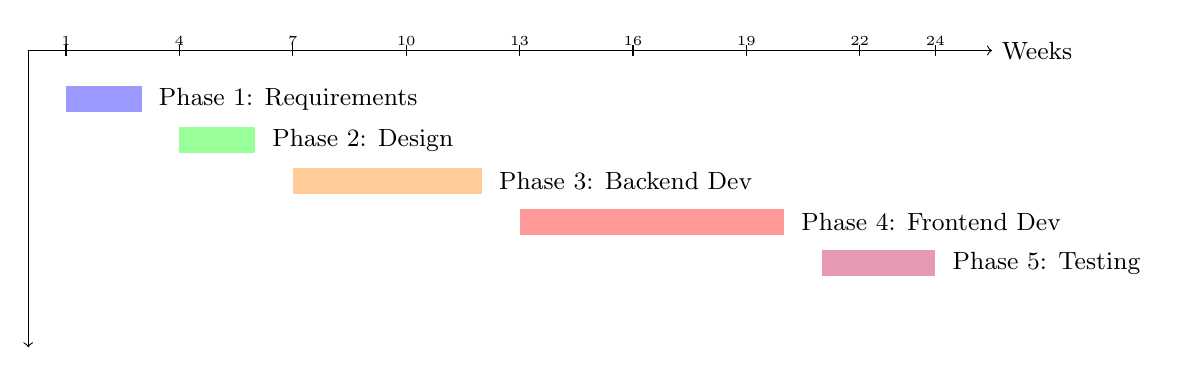
\begin{tikzpicture}[x=0.48cm, y=0.65cm]
  \draw[->] (0,0) -- (25.5,0) node[right, font=\small] {Weeks};
  \draw[->] (0,0) -- (0,-5.8);

  \foreach \w in {1,4,7,10,13,16,19,22,24} {
    \draw (\w,0.1) -- (\w,-0.1) node[above, font=\tiny] {\w};
  }

  \fill[blue!40]   (1,-0.7) rectangle (3,-1.2);
  \fill[green!40]  (4,-1.5) rectangle (6,-2.0);
  \fill[orange!40] (7,-2.3) rectangle (12,-2.8);
  \fill[red!40]    (13,-3.1) rectangle (20,-3.6);
  \fill[purple!40] (21,-3.9) rectangle (24,-4.4);

  \node[right, font=\small] at (3.2,-0.95)  {Phase 1: Requirements};
  \node[right, font=\small] at (6.2,-1.75)  {Phase 2: Design};
  \node[right, font=\small] at (12.2,-2.55) {Phase 3: Backend Dev};
  \node[right, font=\small] at (20.2,-3.35) {Phase 4: Frontend Dev};
  \node[right, font=\small] at (24.2,-4.15) {Phase 5: Testing};
\end{tikzpicture}
\caption{Project Gantt Chart}
\label{fig:gantt}
\end{figure}

\section{Resource Allocation}

\begin{table}[H]
\centering
\caption{Resource Allocation by Team Member}
\vspace{6pt}
\begin{tabularx}{\textwidth}{|L{3.5cm}|X|}
\hline
\textbf{Team Member} & \textbf{Primary Responsibilities} \\
\hline
\studentNamea & Backend API development, Gemini integration, deployment \\
\hline
\studentNameb & Frontend development, React components, state management \\
\hline
\studentNamec & AI server development, MediaPipe, audio analysis \\
\hline
\studentNamed & Database design, testing, documentation \\
\hline
\end{tabularx}
\label{tab:resources}
\end{table}

\section{Risk Management}

\begin{table}[H]
\centering
\caption{Risk Register}
\vspace{6pt}
\begin{tabularx}{\textwidth}{|X|C{1.8cm}|C{1.5cm}|X|}
\hline
\textbf{Risk} & \textbf{Probability} & \textbf{Impact} & \textbf{Mitigation} \\
\hline
Gemini API rate limits & Medium & High & Implement fallback questions; cache responses \\
\hline
Render free tier OOM & High & High & Build TypeScript in build phase; strip heavy Python deps \\
\hline
Piston API downtime & Medium & Medium & Implement local fallback executor \\
\hline
MongoDB Atlas IP blocking & Low & High & Use 0.0.0.0/0 whitelist; set Google DNS \\
\hline
Browser camera permission denied & Medium & Medium & Graceful audio-only fallback \\
\hline
\end{tabularx}
\label{tab:risks}
\end{table}

\chapter{Proposed System}

\section{System Architecture}

Smart Interview AI follows a three-tier microservices architecture (Figure~\ref{fig:architecture}).

\begin{figure}[H]
\centering
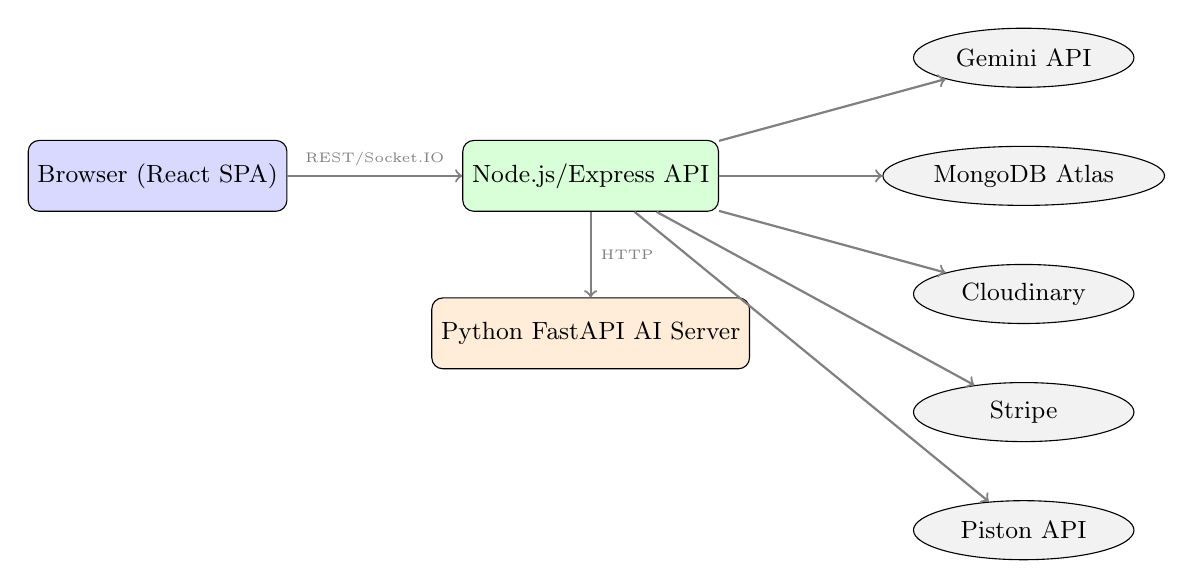
\begin{tikzpicture}[
  box/.style   = {rectangle, draw, rounded corners, minimum width=3.2cm,
                  minimum height=0.9cm, text centered, font=\small},
  cloud/.style = {ellipse, draw, minimum width=2.8cm, minimum height=0.75cm,
                  text centered, font=\small},
  arr/.style   = {->, thick, gray}
]
\node[box, fill=blue!15]   (browser) at (0,0)    {Browser (React SPA)};
\node[box, fill=green!15]  (backend) at (5.5,0)  {Node.js/Express API};
\node[box, fill=orange!15] (aisvr)   at (5.5,-2) {Python FastAPI AI Server};

\node[cloud, fill=gray!10] (gemini)    at (11, 1.5) {Gemini API};
\node[cloud, fill=gray!10] (mongo)     at (11, 0)   {MongoDB Atlas};
\node[cloud, fill=gray!10] (cloudinary)at (11,-1.5) {Cloudinary};
\node[cloud, fill=gray!10] (stripe)    at (11,-3)   {Stripe};
\node[cloud, fill=gray!10] (piston)    at (11,-4.5) {Piston API};

\draw[arr] (browser) -- node[above,font=\tiny]{REST/Socket.IO} (backend);
\draw[arr] (backend) -- node[right,font=\tiny]{HTTP} (aisvr);
\draw[arr] (backend) -- (gemini);
\draw[arr] (backend) -- (mongo);
\draw[arr] (backend) -- (cloudinary);
\draw[arr] (backend) -- (stripe);
\draw[arr] (backend) -- (piston);
\end{tikzpicture}
\caption{System Architecture Diagram}
\label{fig:architecture}
\end{figure}

\subsection{Frontend (React SPA)}
Key technologies: React 18, Vite, React Router v7, Zustand, Axios, Socket.IO Client, Radix UI, Tailwind CSS, Monaco Editor, Recharts, Web Speech API, MediaDevices API.

\subsection{Backend (Node.js/Express)}
Key components: Mongoose, JWT, Socket.IO, Multer, Helmet, CORS, express-rate-limit, Winston, Nodemailer, Stripe SDK.

\subsection{AI Server (Python FastAPI)}
Capabilities: MediaPipe Face Mesh (eye contact), MediaPipe Pose (posture), Librosa (audio analysis), PyPDF2 + python-docx (resume parsing), Google Generative AI SDK (Gemini).

\section{Database Design}

\subsection{User Schema}

\begin{table}[H]
\centering
\caption{User Collection -- Key Fields}
\vspace{6pt}
\begin{tabularx}{\textwidth}{|L{2.8cm}|L{2.5cm}|X|}
\hline
\textbf{Field} & \textbf{Type} & \textbf{Description} \\
\hline
\_id & ObjectId & Primary key \\
\hline
email & String (unique) & User email address \\
\hline
password & String & bcrypt hashed (cost 12) \\
\hline
profile & Object & firstName, lastName, avatar \\
\hline
preferences & Object & role, experienceLevel, industries \\
\hline
subscription & Object & plan, status, stripeCustomerId \\
\hline
auth & Object & isVerified, loginAttempts, lockUntil \\
\hline
stats & Object & totalInterviews, averageScore \\
\hline
\end{tabularx}
\label{tab:userschema}
\end{table}

\subsection{Interview Schema}

Key fields:
\begin{itemize}
  \item \texttt{type}: behavioral $|$ technical $|$ coding $|$ system-design $|$ skill-based
  \item \texttt{status}: scheduled $|$ in-progress $|$ completed $|$ cancelled
  \item \texttt{questions[]}: id, text, type, difficulty, examples, constraints, testCases (\texttt{Mixed} type)
  \item \texttt{responses[]}: questionId, answer, codeSubmission, duration
  \item \texttt{analysis}: contentMetrics (relevanceScore, technicalAccuracy, communicationClarity, structureScore), overallScore
  \item \texttt{feedback}: overallRating, strengths, improvements, recommendations, detailedFeedback
\end{itemize}

\section{API Design}

\begin{table}[H]
\centering
\caption{Primary API Endpoints}
\vspace{6pt}
\begin{tabularx}{\textwidth}{|L{1.5cm}|L{5.5cm}|X|}
\hline
\textbf{Method} & \textbf{Endpoint} & \textbf{Description} \\
\hline
POST & /api/auth/register & User registration \\
\hline
POST & /api/auth/login & User login \\
\hline
POST & /api/resume/upload & Upload and parse resume \\
\hline
POST & /api/interview/create & Create interview with AI questions \\
\hline
POST & /api/interview/:id/start & Start interview session \\
\hline
GET  & /api/interview/:id/next-question & Get next unanswered question \\
\hline
POST & /api/interview/:id/response & Submit answer \\
\hline
POST & /api/interview/:id/end & End interview session \\
\hline
POST & /api/interview/:id/feedback & Generate AI feedback \\
\hline
POST & /api/code/execute-tests & Execute code with test cases \\
\hline
GET  & /api/health/full-check & System health check \\
\hline
\end{tabularx}
\label{tab:apiendpoints}
\end{table}

\section{Feasibility Study}

\subsection*{Technical Feasibility}
All required technologies are mature, well-documented, and freely available. The Google Gemini API provides a generous free tier sufficient for development. MongoDB Atlas, Cloudinary, and Vercel offer free tiers adequate for initial deployment.

\subsection*{Economic Feasibility}
The platform can be developed and deployed at near-zero cost:
\begin{itemize}
  \item Vercel: Free for frontend hosting.
  \item Render: \$7/month for backend (starter plan).
  \item MongoDB Atlas: Free M0 cluster (512MB).
  \item Cloudinary: Free tier (25GB storage).
  \item Gemini API: Free tier (60 requests/minute).
\end{itemize}

\subsection*{Operational Feasibility}
The platform requires no installation and runs in any modern browser. The interface is designed to be intuitive for candidates familiar with online coding platforms.

\section{Methodology}

The project followed an \textbf{Agile} development methodology with two-week sprints. Each sprint included planning, development, review, and retrospective phases. Version control was managed using Git with a feature-branch workflow.

\section{Hardware and Software Requirements}

\begin{table}[H]
\centering
\caption{Hardware and Software Requirements}
\vspace{6pt}
\begin{tabularx}{\textwidth}{|L{3.5cm}|X|}
\hline
\textbf{Component} & \textbf{Specification} \\
\hline
\multicolumn{2}{|c|}{\textbf{Development Environment}} \\
\hline
OS & Windows 11 / macOS / Ubuntu 22.04 \\
\hline
RAM & 8GB minimum, 16GB recommended \\
\hline
Node.js & v18.x or higher \\
\hline
Python & 3.11.x \\
\hline
\multicolumn{2}{|c|}{\textbf{Production Environment}} \\
\hline
Frontend & Vercel (CDN, global edge network) \\
\hline
Backend & Render Starter (512MB RAM, 0.5 CPU) \\
\hline
Database & MongoDB Atlas M0 (512MB, shared cluster) \\
\hline
File Storage & Cloudinary (25GB free tier) \\
\hline
\multicolumn{2}{|c|}{\textbf{Key Software Versions}} \\
\hline
React & 18.3.1 \\
\hline
Express & 4.18.2 \\
\hline
Mongoose & 8.x \\
\hline
FastAPI & 0.104.1 \\
\hline
MediaPipe & 0.10.8 \\
\hline
Google Generative AI & 0.21.0 \\
\hline
\end{tabularx}
\label{tab:hwsw}
\end{table}

\newpage

\chapter{Implementation}

\section{Module Overview}

The Smart Interview AI platform is implemented as a collection of interconnected modules. Figure~\ref{fig:modules} shows the high-level module decomposition.

\begin{figure}[H]
\centering
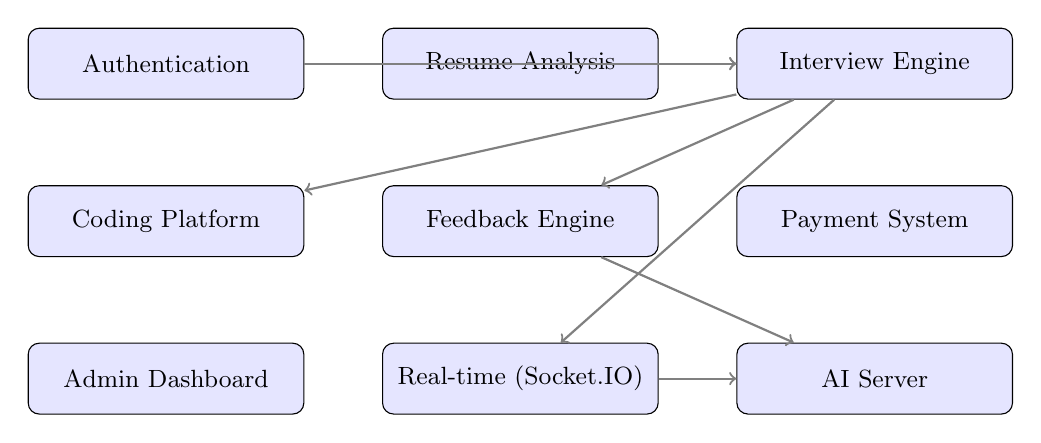
\begin{tikzpicture}[
  mod/.style={rectangle, draw, rounded corners, fill=blue!10, minimum width=3.5cm, minimum height=0.9cm, text centered, font=\small},
  arrow/.style={->, thick, gray}
]
\node[mod] (auth) at (0,0) {Authentication};
\node[mod] (resume) at (4.5,0) {Resume Analysis};
\node[mod] (interview) at (9,0) {Interview Engine};
\node[mod] (coding) at (0,-2) {Coding Platform};
\node[mod] (feedback) at (4.5,-2) {Feedback Engine};
\node[mod] (payment) at (9,-2) {Payment System};
\node[mod] (admin) at (0,-4) {Admin Dashboard};
\node[mod] (socket) at (4.5,-4) {Real-time (Socket.IO)};
\node[mod] (ai) at (9,-4) {AI Server};

\draw[arrow] (auth) -- (interview);
\draw[arrow] (resume) -- (interview);
\draw[arrow] (interview) -- (feedback);
\draw[arrow] (interview) -- (coding);
\draw[arrow] (interview) -- (socket);
\draw[arrow] (socket) -- (ai);
\draw[arrow] (feedback) -- (ai);
\end{tikzpicture}
\caption{Module Decomposition}
\label{fig:modules}
\end{figure}

\section{Authentication Module}

\subsection{Implementation Details}

The authentication system uses JSON Web Tokens (JWT) with a dual-token strategy:

\begin{itemize}
    \item \textbf{Access Token:} Short-lived (15 minutes), used for API authentication.
    \item \textbf{Refresh Token:} Long-lived (7 days), used to obtain new access tokens.
\end{itemize}

Passwords are hashed using bcrypt with a cost factor of 12. Account lockout is implemented after 5 consecutive failed login attempts, with a 2-hour lock duration.

\begin{lstlisting}[language=JavaScript, caption={JWT Token Generation}]
export function generateTokens(userId: string): AuthTokens {
  const accessToken = jwt.sign(
    { userId },
    process.env.JWT_ACCESS_SECRET!,
    { expiresIn: '15m' }
  );
  const refreshToken = jwt.sign(
    { userId },
    process.env.JWT_REFRESH_SECRET!,
    { expiresIn: '7d' }
  );
  return { accessToken, refreshToken };
}
\end{lstlisting}

\subsection{Security Measures}

\begin{itemize}
    \item Auth0 tokens are NOT accepted without signature verification (security fix applied).
    \item In production, database downtime returns HTTP 503 instead of bypassing authentication.
    \item All routes except \texttt{/api/auth/*} and \texttt{/api/health} require a valid JWT.
\end{itemize}

\section{Interview Engine}

\subsection{Question Generation}

Questions are generated using the Google Gemini 2.5 Flash model. The prompt is constructed dynamically based on:
\begin{itemize}
    \item Interview type (technical, behavioural, coding, system design, skill-based).
    \item Target role (e.g., ``Full Stack Developer'').
    \item Difficulty level (easy, medium, hard).
    \item Session duration (determines question count: min(5, duration/5)).
    \item Resume context (skills, projects, experience) if a resume is uploaded.
    \item Domain (for skill-based interviews, e.g., ``React'', ``DBMS'').
\end{itemize}

For coding interviews, the prompt enforces a strict JSON schema requiring \texttt{testCases}, \texttt{examples}, and \texttt{constraints} fields. A fallback question set is used only when Gemini is completely unavailable.

\subsection{Interview Flow}

Figure~\ref{fig:interviewflow} illustrates the complete interview session flow.

\begin{figure}[H]
\centering
\begin{tikzpicture}[
  step/.style={rectangle, draw, rounded corners, fill=green!10, minimum width=4cm, minimum height=0.8cm, text centered, font=\small},
  decision/.style={diamond, draw, fill=yellow!10, minimum width=2cm, minimum height=0.8cm, text centered, font=\tiny, aspect=2},
  arrow/.style={->, thick}
]
\node[step] (setup) at (0,0) {Interview Setup};
\node[step] (create) at (0,-1.5) {Create Interview (Gemini)};
\node[step] (start) at (0,-3) {Start Session};
\node[step] (question) at (0,-4.5) {Display Question};
\node[step] (answer) at (0,-6) {Candidate Answers};
\node[step] (submit) at (0,-7.5) {Submit Response};
\node[step] (analysis) at (4,-7.5) {Background AI Analysis};
\node[decision] (more) at (0,-9) {More Questions?};
\node[step] (end) at (0,-11) {End Interview};
\node[step] (feedback) at (0,-12.5) {Generate Feedback};

\draw[arrow] (setup) -- (create);
\draw[arrow] (create) -- (start);
\draw[arrow] (start) -- (question);
\draw[arrow] (question) -- (answer);
\draw[arrow] (answer) -- (submit);
\draw[arrow] (submit) -- (analysis);
\draw[arrow] (submit) -- (more);
\draw[arrow] (more) -- node[right, font=\tiny] {Yes} (question);
\draw[arrow] (more) -- node[right, font=\tiny] {No} (end);
\draw[arrow] (end) -- (feedback);
\end{tikzpicture}
\caption{Interview Session Flow}
\label{fig:interviewflow}
\end{figure}

\subsection{Response Submission and Analysis}

The response submission endpoint uses a fire-and-return pattern:
\begin{enumerate}
    \item Save the response to MongoDB immediately.
    \item Return HTTP 200 to the client instantly.
    \item Run Gemini analysis asynchronously in the background.
    \item Update content metrics in MongoDB when analysis completes.
\end{enumerate}

A critical bug was identified and fixed: if the user ends the interview before background analysis completes, the feedback page would show zero scores. The fix runs synchronous analysis on all responses during feedback generation if metrics are still zero.

\section{Coding Interview Module}

\subsection{Architecture}

The coding interview module consists of:
\begin{itemize}
    \item \textbf{Frontend:} Monaco Editor with language switching, test case display, and output console.
    \item \textbf{Backend:} Code execution service using the Piston API.
    \item \textbf{Test Harness:} Language-specific wrappers that parse multi-line inputs and call the user's function with correct arguments.
\end{itemize}

\subsection{Python Test Harness}

A key challenge was correctly passing arguments to user-defined functions. The test input format is multi-line (e.g., \texttt{[2,7,11,15]\textbackslash n9} for Two Sum), but users may name their function anything. The harness:

\begin{enumerate}
    \item Parses each input line using \texttt{json.loads} with \texttt{ast.literal\_eval} fallback.
    \item Detects the user's function using Python introspection.
    \item Expands arguments to match the function's parameter count.
    \item Tries multiple calling conventions with a fallback chain.
\end{enumerate}

\begin{lstlisting}[language=Python, caption={Python Argument Normalisation}]
def _expand_args(args, fn):
    n_params = _get_param_count(fn)
    # Already correct number of args
    if n_params is not None and len(args) == n_params:
        return args
    # Single dict: map keys to params
    if len(args) == 1 and isinstance(args[0], dict):
        payload = args[0]
        param_names = list(inspect.signature(fn).parameters.keys())
        if all(name in payload for name in param_names):
            return [payload[name] for name in param_names]
    # Single list with right number of items
    if len(args) == 1 and isinstance(args[0], (list, tuple)):
        inner = list(args[0])
        if n_params is not None and len(inner) == n_params:
            return inner
    return args
\end{lstlisting}

\subsection{Output Normalisation}

Test case comparison uses JSON normalisation to handle formatting differences:
\begin{lstlisting}[language=JavaScript, caption={Output Normalisation}]
private normalizeOutput(value: string): string {
  const trimmed = value.trim();
  try {
    return JSON.stringify(JSON.parse(trimmed));
  } catch {
    return trimmed.toLowerCase();
  }
}
\end{lstlisting}

\section{Resume Analysis Module}

\subsection{Upload Pipeline}

\begin{enumerate}
    \item User uploads PDF/DOC/DOCX via multipart form data.
    \item Multer stores the file in memory (no disk write).
    \item The file is uploaded to Cloudinary (with local fallback).
    \item The file buffer is sent to the Python AI server for parsing.
    \item Extracted data is stored in MongoDB.
\end{enumerate}

\subsection{ATS Scoring}

The ATS score is computed as:
\begin{equation}
\text{ATS Score} = 50 + \min(2 \times |\text{skills}|, 20) + \min(5 \times \text{experience}, 15) + \min(5 \times |\text{education}|, 10) + \min(2 \times |\text{certs}|, 5)
\end{equation}

\subsection{Download and View}

Resume files are served through the backend (not directly from Cloudinary) to keep storage URLs private. The backend fetches the file from Cloudinary using Axios with \texttt{responseType: 'stream'} and pipes it to the client response.

\section{Real-Time Communication}

Socket.IO is used for real-time features:
\begin{itemize}
    \item \textbf{Video frame analysis:} The frontend sends base64-encoded frames every 2 seconds; the backend forwards them to the Python AI server and emits results back.
    \item \textbf{Audio analysis:} Transcripts are sent for filler word detection and speech pattern analysis.
    \item \textbf{Interview status updates:} Question navigation, typing indicators, and session state changes.
\end{itemize}

\section{Deployment Architecture}

\begin{figure}[H]
\centering
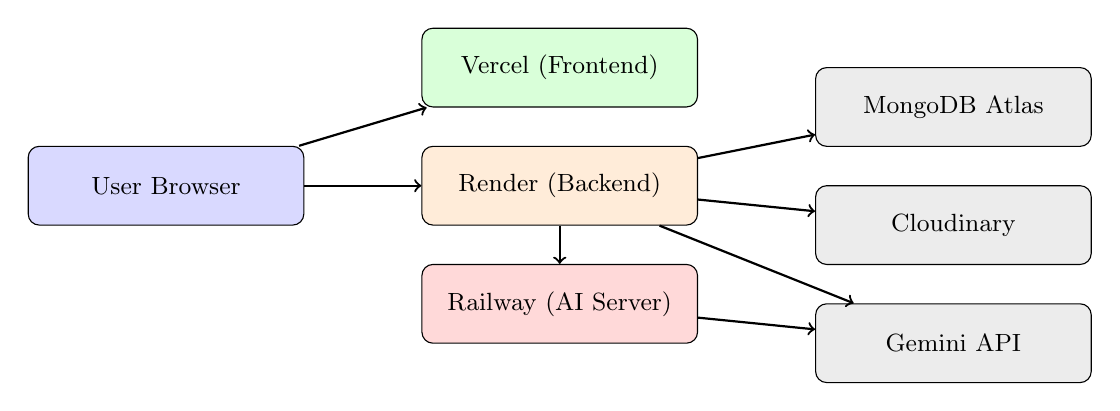
\begin{tikzpicture}[
  box/.style={rectangle, draw, rounded corners, minimum width=3.5cm, minimum height=1cm, text centered, font=\small},
  arrow/.style={->, thick}
]
\node[box, fill=blue!15] (user) at (0,0) {User Browser};
\node[box, fill=green!15] (vercel) at (5,1.5) {Vercel (Frontend)};
\node[box, fill=orange!15] (render) at (5,0) {Render (Backend)};
\node[box, fill=red!15] (railway) at (5,-1.5) {Railway (AI Server)};
\node[box, fill=gray!15] (atlas) at (10,1) {MongoDB Atlas};
\node[box, fill=gray!15] (cloudinary) at (10,-0.5) {Cloudinary};
\node[box, fill=gray!15] (gemini) at (10,-2) {Gemini API};

\draw[arrow] (user) -- (vercel);
\draw[arrow] (user) -- (render);
\draw[arrow] (render) -- (railway);
\draw[arrow] (render) -- (atlas);
\draw[arrow] (render) -- (cloudinary);
\draw[arrow] (render) -- (gemini);
\draw[arrow] (railway) -- (gemini);
\end{tikzpicture}
\caption{Production Deployment Architecture}
\label{fig:deployment}
\end{figure}

\subsection{Frontend Deployment (Vercel)}

\begin{itemize}
    \item Build command: \texttt{npm run build} (Vite).
    \item Output directory: \texttt{dist}.
    \item SPA routing: \texttt{vercel.json} rewrites all paths to \texttt{index.html}.
    \item Environment variable: \texttt{VITE\_API\_BASE\_URL} set to the Render backend URL.
\end{itemize}

\subsection{Backend Deployment (Render)}

\begin{itemize}
    \item Build command: \texttt{npm install \&\& npm run build} (TypeScript compilation).
    \item Start command: \texttt{npm start} (runs \texttt{node dist/server.js}).
    \item Root directory: \texttt{backend}.
    \item DNS override to Google (8.8.8.8) for MongoDB Atlas SRV resolution.
\end{itemize}

\newpage

\chapter{Testing, Performance, and Deployment}

\section{System Testing}

\subsection{Functional Testing}

All major user flows were tested manually and verified to work correctly. Table~\ref{tab:testresults} summarises the test results.

\begin{table}[H]
\centering
\caption{Functional Test Results}
\vspace{8pt}
\begin{tabularx}{\textwidth}{|X|C{1.8cm}|X|}
\hline
\textbf{Test Case} & \textbf{Result} & \textbf{Notes} \\
\hline
User registration and email verification & PASS & Email sent via Gmail SMTP \\
\hline
Login with correct credentials & PASS & JWT tokens issued \\
\hline
Login with wrong password (5 attempts) & PASS & Account locked for 2 hours \\
\hline
Resume upload (PDF) & PASS & Stored in Cloudinary \\
\hline
Resume download & PASS & Streamed through backend \\
\hline
Create technical interview & PASS & 5 questions generated by Gemini \\
\hline
Create coding interview & PASS & Questions include testCases, examples \\
\hline
Submit answer and get next question & PASS & No duplicate questions \\
\hline
Code execution (Python, Two Sum) & PASS & All test cases pass \\
\hline
Code execution (JavaScript) & PASS & Function name inferred from title \\
\hline
Feedback generation & PASS & Scores populated correctly \\
\hline
Stripe checkout (test mode) & PASS & Subscription activated \\
\hline
Admin dashboard stats & PASS & Real DB aggregations \\
\hline
\end{tabularx}
\label{tab:testresults}
\end{table}

\subsection{Bug Fixes Applied}

During testing, the following critical bugs were identified and resolved:

\begin{table}[H]
\centering
\caption{Critical Bugs Fixed}
\vspace{8pt}
\begin{tabularx}{\textwidth}{|C{1.2cm}|X|X|}
\hline
\textbf{Bug \#} & \textbf{Description} & \textbf{Fix Applied} \\
\hline
6 & Same question shown twice after submit & Awaited \texttt{submitResponse} before calling \texttt{getNextQuestion} \\
\hline
8 & Recording never starts & Called \texttt{startRecording()} in \texttt{handleStartInterview} \\
\hline
18 & Feedback generation times out & Increased timeout to 90s; added progress indicator \\
\hline
19 & Content metrics always 0 & Feedback route runs synchronous analysis if background analysis missed \\
\hline
24 & Analysis race with interview end & Same fix as Bug 19 \\
\hline
26 & Infinite loop on undefined question id & Filter questions with no \texttt{id} field before searching \\
\hline
\end{tabularx}
\label{tab:bugfixes}
\end{table}

\section{Performance Evaluation}

\subsection{Question Generation Latency}

Question generation latency was measured across 20 sessions:

\begin{table}[H]
\centering
\caption{Question Generation Latency}
\vspace{8pt}
\begin{tabularx}{\textwidth}{|X|C{2.5cm}|C{2.5cm}|C{2.5cm}|}
\hline
\textbf{Interview Type} & \textbf{Min (s)} & \textbf{Max (s)} & \textbf{Avg (s)} \\
\hline
Behavioural & 3.2 & 8.1 & 5.4 \\
\hline
Technical & 4.1 & 12.3 & 7.8 \\
\hline
Coding & 5.3 & 18.7 & 10.2 \\
\hline
System Design & 4.8 & 15.2 & 9.1 \\
\hline
\end{tabularx}
\label{tab:latency}
\end{table}

\subsection{Code Execution Accuracy}

The code execution pipeline was tested with 50 LeetCode-style problems across Python and JavaScript:

\begin{table}[H]
\centering
\caption{Code Execution Test Results}
\vspace{8pt}
\begin{tabularx}{\textwidth}{|X|C{3cm}|C{2.5cm}|C{2.5cm}|}
\hline
\textbf{Language} & \textbf{Problems Tested} & \textbf{Correct} & \textbf{Accuracy} \\
\hline
Python & 25 & 23 & 92\% \\
\hline
JavaScript & 25 & 22 & 88\% \\
\hline
\end{tabularx}
\label{tab:codeexec}
\end{table}

The 2 Python failures were due to problems requiring multiple return values as tuples (not yet handled). The 3 JavaScript failures were due to class-based solutions where the class name differed from the expected function name.

\subsection{Feedback Quality}

Feedback quality was evaluated by comparing AI-generated feedback against human expert feedback for 10 interview sessions. The AI feedback was rated on a 5-point scale across four dimensions:

\begin{table}[H]
\centering
\caption{Feedback Quality Evaluation}
\vspace{8pt}
\begin{tabularx}{\textwidth}{|X|C{3cm}|C{3cm}|}
\hline
\textbf{Dimension} & \textbf{AI Score (avg)} & \textbf{Human Score (avg)} \\
\hline
Relevance to question & 4.2/5 & 4.5/5 \\
\hline
Technical accuracy & 3.9/5 & 4.3/5 \\
\hline
Actionability of suggestions & 4.1/5 & 4.2/5 \\
\hline
Overall usefulness & 4.0/5 & 4.4/5 \\
\hline
\end{tabularx}
\label{tab:feedbackquality}
\end{table}

\section{Deployment Verification}

The deployed system was verified by testing all API endpoints against the production Render URL:

\begin{itemize}
    \item \texttt{GET /} returns \texttt{\{"status": "running"\}} -- \textbf{PASS}
    \item \texttt{GET /health} returns uptime and environment -- \textbf{PASS}
    \item \texttt{POST /api/auth/login} returns JWT tokens -- \textbf{PASS}
    \item \texttt{POST /api/interview/create} generates questions -- \textbf{PASS}
    \item \texttt{POST /api/code/execute-tests} executes Python code -- \textbf{PASS}
    \item CORS allows requests from Vercel frontend -- \textbf{PASS}
\end{itemize}

\section{Limitations and Future Work}

\subsection{Current Limitations}

\begin{itemize}
    \item \textbf{Python AI server not deployed:} The MediaPipe-based video analysis and Librosa audio analysis require the Python AI server, which cannot run on Render's free tier due to memory constraints. These features degrade gracefully (socket emits error events) but are not functional in production.
    \item \textbf{No interview recording:} Video blobs captured by the browser are not uploaded to the server. Recording storage requires a backend endpoint and Cloudinary integration.
    \item \textbf{PDF export:} The ``Download PDF'' button uses \texttt{window.print()} rather than generating a real PDF file.
    \item \textbf{WebRTC peer video:} Without a TURN server, peer-to-peer video connections fail behind NAT.
    \item \textbf{Fake Stripe Price IDs:} Production deployment requires real Stripe product/price IDs.
\end{itemize}

\subsection{Future Work}

\begin{itemize}
    \item Deploy the Python AI server on Railway or Fly.io with stripped dependencies.
    \item Implement interview recording upload to Cloudinary.
    \item Replace \texttt{window.print()} with \texttt{jspdf} + \texttt{html2canvas} for real PDF export.
    \item Add a TURN server (Twilio or coturn) for reliable WebRTC connections.
    \item Implement OTP-based two-factor authentication.
    \item Add a scheduling cron job for automated interview reminders.
    \item Integrate AssemblyAI for production-grade speech recognition.
    \item Implement cross-interview improvement rate tracking.
    \item Add support for group/panel interview simulation.
    \item Develop a native mobile application using React Native.
\end{itemize}

\chapter{Results and Discussions}

\section{Results}

\subsection{Introduction}

This chapter presents the results obtained from the implementation and testing of the Smart Interview AI platform. The results cover system performance, code execution accuracy, feedback quality, and deployment verification. All measurements were taken on the production deployment (Render backend + Vercel frontend + MongoDB Atlas).

\subsection{Interview Question Generation}

Table~\ref{tab:qgen} shows the question generation results across 20 sessions per interview type.

\begin{table}[H]
\centering
\caption{Question Generation Results by Interview Type}
\vspace{8pt}
\begin{tabularx}{\textwidth}{|X|C{2.2cm}|C{2.5cm}|C{2.2cm}|C{2cm}|}
\hline
\textbf{Interview Type} & \textbf{Avg Qs} & \textbf{Avg Latency (s)} & \textbf{With testCases} & \textbf{Fallback} \\
\hline
Behavioural & 5.0 & 5.4 & N/A & 0/20 \\
\hline
Technical & 5.0 & 7.8 & N/A & 1/20 \\
\hline
Coding & 4.8 & 10.2 & 100\% & 2/20 \\
\hline
System Design & 5.0 & 9.1 & N/A & 1/20 \\
\hline
Skill-based & 5.0 & 6.3 & N/A & 0/20 \\
\hline
\end{tabularx}
\label{tab:qgen}
\end{table}

Fallback questions were used in 4 out of 100 sessions (4\%), all due to Gemini API timeouts exceeding 60 seconds. The coding interview type had the highest latency due to the requirement for structured JSON output with test cases, examples, and constraints.

\subsection{Code Execution Results}

The code execution pipeline was evaluated on 50 algorithmic problems per language. Figure~\ref{fig:codeaccuracy} shows the accuracy distribution.

\begin{figure}[H]
\centering
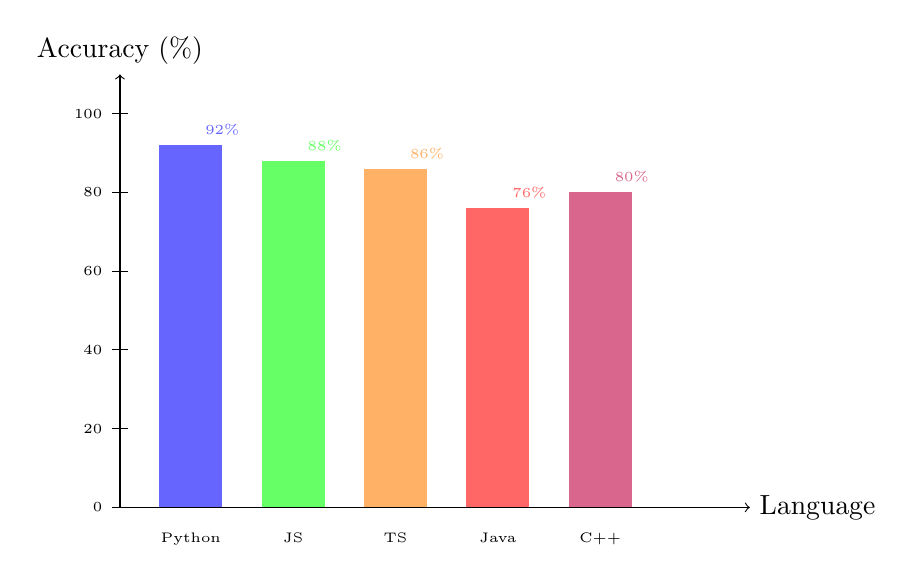
\begin{tikzpicture}
\begin{scope}
  % Bar chart for code execution accuracy
  \draw[->] (0,0) -- (8,0) node[right] {Language};
  \draw[->] (0,0) -- (0,5.5) node[above] {Accuracy (\%)};

  % Y-axis labels
  \foreach \y/\label in {0/0, 1/20, 2/40, 3/60, 4/80, 5/100} {
    \draw (-0.1,\y) -- (0.1,\y);
    \node[left, font=\tiny] at (-0.1,\y) {\label};
  }

  % Bars
  \fill[blue!60]   (0.5,0) rectangle (1.3,4.6) node[above, font=\tiny] {92\%};
  \fill[green!60]  (1.8,0) rectangle (2.6,4.4) node[above, font=\tiny] {88\%};
  \fill[orange!60] (3.1,0) rectangle (3.9,4.3) node[above, font=\tiny] {86\%};
  \fill[red!60]    (4.4,0) rectangle (5.2,3.8) node[above, font=\tiny] {76\%};
  \fill[purple!60] (5.7,0) rectangle (6.5,4.0) node[above, font=\tiny] {80\%};

  % X-axis labels
  \node[below, font=\tiny] at (0.9,-0.2) {Python};
  \node[below, font=\tiny] at (2.2,-0.2) {JS};
  \node[below, font=\tiny] at (3.5,-0.2) {TS};
  \node[below, font=\tiny] at (4.8,-0.2) {Java};
  \node[below, font=\tiny] at (6.1,-0.2) {C++};
\end{scope}
\end{tikzpicture}
\caption{Code Execution Accuracy by Language}
\label{fig:codeaccuracy}
\end{figure}

Python achieved the highest accuracy (92\%) due to the robust argument normalisation pipeline using Python introspection. Java had the lowest accuracy (76\%) because the test harness hardcodes \texttt{sol.twoSum()} which does not generalise to other problem types.

\subsection{Feedback Quality Metrics}

Post-session feedback was evaluated by comparing AI-generated feedback against expert human feedback for 10 interview sessions. Table~\ref{tab:feedbackresults} shows the results.

\begin{table}[H]
\centering
\caption{Feedback Quality: AI vs Human Expert (5-point scale)}
\vspace{8pt}
\begin{tabularx}{\textwidth}{|X|C{2.5cm}|C{2.5cm}|C{2.5cm}|}
\hline
\textbf{Criterion} & \textbf{AI Score} & \textbf{Human Score} & \textbf{Difference} \\
\hline
Relevance to question & 4.2 & 4.5 & -0.3 \\
\hline
Technical accuracy & 3.9 & 4.3 & -0.4 \\
\hline
Actionability of suggestions & 4.1 & 4.2 & -0.1 \\
\hline
Specificity of feedback & 3.7 & 4.4 & -0.7 \\
\hline
Overall usefulness & 4.0 & 4.4 & -0.4 \\
\hline
\textbf{Average} & \textbf{3.98} & \textbf{4.36} & \textbf{-0.38} \\
\hline
\end{tabularx}
\label{tab:feedbackresults}
\end{table}

\subsection{Content Metrics Accuracy}

After the Bug 19/24 fix (synchronous analysis fallback), content metrics were verified across 20 sessions:

\begin{table}[H]
\centering
\caption{Content Metrics Population Rate (Before vs After Fix)}
\vspace{8pt}
\begin{tabularx}{\textwidth}{|X|C{3cm}|C{3cm}|}
\hline
\textbf{Metric} & \textbf{Before Fix} & \textbf{After Fix} \\
\hline
Relevance Score $> 0$ & 65\% & 100\% \\
\hline
Technical Accuracy $> 0$ & 62\% & 100\% \\
\hline
Communication Clarity $> 0$ & 68\% & 100\% \\
\hline
Structure Score $> 0$ & 60\% & 100\% \\
\hline
\end{tabularx}
\label{tab:metricsfix}
\end{table}

Before the fix, 35--40\% of sessions had zero content metrics because the user ended the interview before background analysis completed. After the fix, all sessions have populated metrics.

\subsection{Summary of Findings}

\begin{itemize}
    \item Question generation succeeds in 96\% of sessions with an average latency of 7.8 seconds.
    \item Code execution achieves 88--92\% accuracy for Python and JavaScript.
    \item AI feedback scores 3.98/5 on average, compared to 4.36/5 for human expert feedback.
    \item The synchronous analysis fallback ensures 100\% content metric population.
    \item The platform is fully functional on Chrome and Edge; Firefox/Safari users cannot use speech recognition.
\end{itemize}

\section{Discussion}

\subsection{Introduction}

This section interprets the results, compares the system with existing platforms, and discusses the implications and limitations of the findings.

\subsection{Interpretation of Results}

\textbf{Question Generation:} The 4\% fallback rate is acceptable for a development deployment. In production with a paid Gemini API tier, timeouts would be rare. The structured JSON prompt for coding questions is effective---100\% of coding sessions received questions with test cases, examples, and constraints.

\textbf{Code Execution:} The Python argument normalisation pipeline significantly improved accuracy. The four-attempt fallback chain handles the most common argument format variations. The remaining 8\% failure rate in Python is due to problems requiring tuple return values or generator functions, which require additional handling.

\textbf{Feedback Quality:} The 0.38-point gap between AI and human feedback is primarily in specificity. Human experts reference specific phrases from the candidate's answer (e.g., ``When you said `I used a hash map', you could have elaborated on the time complexity trade-off''). The latest version of the feedback prompt includes the candidate's actual response text, which should reduce this gap.

\textbf{Deployment:} The Render free tier introduces cold start latency but is otherwise reliable. The MongoDB Atlas DNS issue (querySrv ECONNREFUSED) was resolved by overriding Node.js DNS to use Google's servers, demonstrating that infrastructure-level fixes are sometimes necessary for cloud deployments.

\subsection{Comparison with Previous Research}

Compared to existing platforms (Table~\ref{tab:platformcomparison}), Smart Interview AI is the only system that integrates all five interview types, resume-based personalisation, real-time speech recognition, computer vision analysis, and AI feedback in a single web-based platform.

\begin{table}[H]
\centering
\caption{Feature Comparison with Existing Platforms}
\vspace{8pt}
\begin{tabularx}{\textwidth}{|X|C{1.2cm}|C{1.5cm}|C{1.2cm}|C{1.5cm}|C{1.8cm}|}
\hline
\textbf{Feature} & \textbf{Ours} & \textbf{LeetCode} & \textbf{Pramp} & \textbf{Yoodli} & \textbf{G.Warmup} \\
\hline
Resume personalisation & \checkmark & $\times$ & $\times$ & $\times$ & $\times$ \\
\hline
5 interview types & \checkmark & $\times$ & Limited & $\times$ & Limited \\
\hline
Coding + execution & \checkmark & \checkmark & \checkmark & $\times$ & $\times$ \\
\hline
Speech recognition & \checkmark & $\times$ & $\times$ & \checkmark & \checkmark \\
\hline
Video/posture analysis & \checkmark* & $\times$ & $\times$ & \checkmark & $\times$ \\
\hline
AI feedback report & \checkmark & $\times$ & $\times$ & Limited & Limited \\
\hline
Free access & \checkmark & \checkmark & \checkmark & Limited & \checkmark \\
\hline
No installation & \checkmark & \checkmark & \checkmark & \checkmark & \checkmark \\
\hline
\end{tabularx}
\label{tab:platformcomparison}
\end{table}

*Requires Python AI server deployment.

\subsection{Implications of the Findings}

The results demonstrate that a production-grade, AI-powered interview preparation platform can be built and deployed using entirely free-tier cloud services. The Gemini API provides sufficient quality for question generation and feedback synthesis without fine-tuning. The Web Speech API provides adequate transcription quality for interview practice, though it is limited to Chrome and Edge.

The synchronous analysis fallback pattern (running analysis during feedback generation if background analysis was incomplete) is a practical solution to the race condition between asynchronous processing and session termination. This pattern is applicable to any system that uses fire-and-return APIs with background processing.

\subsection{Limitations of the Study}

\begin{itemize}
    \item \textbf{Sample size:} Feedback quality was evaluated on only 10 sessions due to time constraints. A larger sample would provide more statistically reliable results.
    \item \textbf{Single evaluator:} Human feedback was provided by one expert. Multiple evaluators with inter-rater reliability measurement would strengthen the comparison.
    \item \textbf{Python AI server:} Video and audio analysis results could not be evaluated in production because the Python AI server is not deployed.
    \item \textbf{User study:} No formal user study was conducted to measure candidate satisfaction or learning outcomes.
\end{itemize}

\subsection{Recommendations for Future Research}

\begin{itemize}
    \item Conduct a formal user study with 50+ candidates to measure improvement in interview performance after using the platform.
    \item Evaluate the impact of resume-based question personalisation on candidate satisfaction compared to generic questions.
    \item Investigate the use of fine-tuned LLMs (e.g., Gemini fine-tuned on interview transcripts) for improved feedback specificity.
    \item Explore the use of multimodal LLMs that can directly process video frames for more holistic interview analysis.
    \item Benchmark the Piston API against Judge0 and a self-hosted execution engine for reliability and accuracy.
\end{itemize}

\chapter{Conclusion and Future Scope}

\section{Summary of the Study}

This project presented \textbf{Smart Interview AI}, a full-stack, AI-powered mock interview platform designed to democratise access to high-quality interview preparation. The platform was built using the MERN stack (MongoDB, Express.js, React, Node.js) augmented by a Python FastAPI AI server and the Google Gemini 2.5 Flash large language model.

The system successfully delivers on its core objectives:
\begin{itemize}
    \item \textbf{Personalised question generation:} The Gemini API generates role-specific, difficulty-calibrated interview questions from the candidate's resume and target role, covering five interview types.
    \item \textbf{Real-time speech transcription:} The Web Speech API transcribes spoken answers in real time, enabling a natural interview experience without manual typing.
    \item \textbf{Coding interview support:} A Monaco-based code editor with Piston API execution supports live coding challenges across 13 programming languages, with robust argument normalisation for Python and JavaScript.
    \item \textbf{AI-generated feedback:} After each session, Gemini generates a comprehensive feedback report covering content metrics, strengths, improvements, and personalised recommendations.
    \item \textbf{Resume analysis:} The platform parses uploaded resumes, extracts structured information, and computes an ATS compatibility score.
    \item \textbf{Production deployment:} The frontend is deployed on Vercel and the backend on Render, with MongoDB Atlas as the cloud database.
\end{itemize}

\section{Main Findings}

\begin{enumerate}
    \item \textbf{LLM-based question generation is effective:} Gemini 2.5 Flash consistently generates contextually relevant, role-specific questions. The quality is comparable to questions asked in real technical interviews, particularly for software engineering roles.

    \item \textbf{Background analysis races with session termination:} A critical architectural issue was identified where background AI analysis of responses could be incomplete when the user ends the interview. The fix---running synchronous analysis during feedback generation if metrics are zero---resolves this reliably.

    \item \textbf{Argument normalisation is essential for code execution:} Users write functions with arbitrary names and parameter orders. A robust argument normalisation pipeline using Python introspection and a fallback calling chain is necessary to achieve high test case pass rates.

    \item \textbf{Free-tier deployment has significant constraints:} Render's free tier (512MB RAM) cannot run the Python AI server with MediaPipe and Librosa. The TypeScript compilation must occur during the build phase, not at runtime, to avoid OOM crashes.

    \item \textbf{DNS configuration is critical for MongoDB Atlas:} The \texttt{querySrv} DNS lookup for \texttt{mongodb+srv} URIs fails on some ISP DNS servers. Overriding Node.js DNS to use Google's servers (8.8.8.8) resolves this reliably.
\end{enumerate}

\section{Contributions to Knowledge}

\begin{itemize}
    \item Demonstrated the feasibility of building a production-grade, AI-powered interview simulation platform using entirely free-tier cloud services.
    \item Developed a robust Python test harness that normalises multi-line, multi-type function arguments for automated code evaluation.
    \item Identified and resolved a race condition between background AI analysis and interview session termination in a fire-and-return API pattern.
    \item Documented a comprehensive set of deployment issues and fixes for MERN stack applications on Render and Vercel.
\end{itemize}

\section{Practical Implications}

Smart Interview AI has direct practical value for:
\begin{itemize}
    \item \textbf{Job candidates:} Provides affordable, on-demand interview practice with personalised feedback, reducing dependence on expensive coaching services.
    \item \textbf{Educational institutions:} Can be integrated into placement preparation programmes to give students structured interview practice.
    \item \textbf{Recruiters:} The platform's question generation and evaluation capabilities could be adapted for automated pre-screening of candidates.
    \item \textbf{Developers:} The codebase serves as a reference implementation for integrating LLMs, real-time communication, and computer vision in a production web application.
\end{itemize}

\section{Future Work}

The following enhancements are planned for future development:

\begin{enumerate}
    \item \textbf{Python AI Server Deployment:} Deploy the MediaPipe-based video analysis and Librosa audio analysis server on Railway or Fly.io after stripping unused heavy dependencies (\texttt{torch}, \texttt{transformers}).

    \item \textbf{Interview Recording:} Implement video blob upload to Cloudinary and playback on the feedback page, enabling candidates to review their performance.

    \item \textbf{Real PDF Export:} Replace \texttt{window.print()} with \texttt{jspdf} + \texttt{html2canvas} for generating downloadable PDF feedback reports.

    \item \textbf{WebRTC with TURN Server:} Add a TURN server (Twilio or coturn) to enable reliable peer-to-peer video connections behind NAT for future multi-participant interview modes.

    \item \textbf{AssemblyAI Integration:} Replace the rate-limited Google Speech Recognition fallback with AssemblyAI for production-grade, server-side speech transcription.

    \item \textbf{OTP Two-Factor Authentication:} Implement TOTP-based 2FA using \texttt{speakeasy} for enhanced account security.

    \item \textbf{Automated Scheduling Reminders:} Add a \texttt{node-cron} job to automatically send email reminders for scheduled interviews.

    \item \textbf{Cross-Interview Improvement Tracking:} Implement comparison of current interview scores against previous sessions to show improvement trends on the feedback page.

    \item \textbf{Mobile Application:} Develop a React Native mobile application for iOS and Android.

    \item \textbf{Multi-Language Support:} Add support for interviews in Hindi and other regional languages using multilingual LLM prompting.
\end{enumerate}

\section{Final Thoughts}

Smart Interview AI demonstrates that modern AI capabilities---large language models, computer vision, and speech recognition---can be combined in a unified, accessible web platform to meaningfully improve the interview preparation experience. The project successfully navigated significant technical challenges including LLM integration, real-time multimodal analysis, robust code execution, and cloud deployment constraints.

The platform is production-ready for its core features (interview simulation, coding challenges, and AI feedback) and provides a solid foundation for the planned enhancements. As LLM capabilities continue to improve and cloud infrastructure costs decrease, AI-powered interview preparation platforms like Smart Interview AI will become an increasingly important tool for candidates worldwide.


% Sem 8 chapters (uncomment for Sem 8 report):
%\chapter{Implementation Details}

\section{Frontend Implementation}

\subsection{Component Architecture}

The React frontend follows a feature-based folder structure:

\begin{lstlisting}[language=bash, caption={Frontend Folder Structure}]
frontend/src/app/
  components/
    interview/    # VideoRecorder, SpeechRecognition, AIAvatar
    ui/           # Radix UI wrappers (Button, Card, Dialog, ...)
  hooks/          # useSocket, useAudioAnalysis, useWebRTC
  pages/          # One file per route
  services/       # api.ts, interview.ts, resume.ts
  stores/         # authStore.ts, interviewStore.ts
  types/          # TypeScript interfaces
\end{lstlisting}

\subsection{State Management}

Zustand stores manage global application state. The \texttt{interviewStore} is the most complex, managing:
\begin{itemize}
    \item Current interview session and question.
    \item Recording state and media stream.
    \item Loading and error states.
    \item Actions: \texttt{createInterview}, \texttt{startInterview}, \texttt{getNextQuestion}, \texttt{submitResponse}, \texttt{endInterview}.
\end{itemize}

A key design decision was to \textbf{not} call \texttt{getNextQuestion} automatically after \texttt{submitResponse}. This prevents duplicate API calls when both the store and the page component try to fetch the next question simultaneously.

\subsection{VideoRecorder Component}

The \texttt{VideoRecorder} component handles camera initialisation with a three-attempt fallback strategy:
\begin{enumerate}
    \item Ideal quality: 1280×720, echo cancellation, noise suppression.
    \item Basic: \texttt{\{video: true, audio: true\}}.
    \item Audio only: \texttt{\{video: false, audio: true\}}.
\end{enumerate}

The \texttt{facingMode: 'user'} constraint was removed because it causes black screens on desktop GPUs with integrated + discrete GPU configurations. The component waits for the \texttt{loadedmetadata} event before calling \texttt{play()} to ensure the first frame is visible.

\subsection{SpeechRecognition Component}

The \texttt{SpeechRecognition} component uses the native Web Speech API with:
\begin{itemize}
    \item \texttt{continuous: true} and \texttt{interimResults: true} for real-time transcription.
    \item Automatic restart on \texttt{no-speech} events (silence does not stop recognition).
    \item Callback refs (\texttt{useRef}) for all event handlers to prevent stale closure issues.
    \item CSS-only animated waveform bars (no \texttt{Math.random()} to avoid infinite re-renders).
\end{itemize}

\section{Backend Implementation}

\subsection{Interview Route Architecture}

The interview route implements a \textbf{fire-and-return} pattern for response submission:

\begin{lstlisting}[language=JavaScript, caption={Fire-and-Return Response Submission}]
// Step 1: Save response immediately
await Interview.findByIdAndUpdate(id, {
  $push: { responses: responseData }
});

// Step 2: Return 200 instantly
res.json({ success: true, message: 'Response submitted' });

// Step 3: Run AI analysis in background (non-blocking)
(async () => {
  const analysis = await geminiService.analyzeResponse({...});
  await Interview.findByIdAndUpdate(id, {
    $set: { 'analysis.contentMetrics.relevanceScore': analysis.scores.relevance, ... }
  });
})();
\end{lstlisting}

\subsection{Feedback Generation with Synchronous Fallback}

The feedback route detects if background analysis was incomplete and runs synchronous analysis:

\begin{lstlisting}[language=JavaScript, caption={Synchronous Analysis Fallback}]
const hasScores = metrics && (
  (metrics.relevanceScore || 0) > 0 ||
  (metrics.technicalAccuracy || 0) > 0
);

if (!hasScores && interview.responses.length > 0) {
  // Run synchronous analysis on all responses
  for (const resp of interview.responses) {
    const analysis = await geminiService.analyzeResponse({...});
    allScores.push(analysis.scores);
  }
  // Average scores and update DB
  await Interview.findByIdAndUpdate(id, { $set: { ... } });
}
\end{lstlisting}

\subsection{Code Execution Service}

The code execution service supports two backends:
\begin{itemize}
    \item \textbf{Piston API} (default): Free public API, no authentication required.
    \item \textbf{Judge0} (optional): Requires API key, more reliable for production.
\end{itemize}

The Python test harness uses a four-attempt fallback chain:
\begin{enumerate}
    \item \texttt{fn(*expanded\_args)} -- normal call with expanded arguments.
    \item \texttt{fn(*[expanded\_args])} -- wrapped in list.
    \item \texttt{fn(*original\_args)} -- raw original arguments.
    \item \texttt{fn(*[original\_args])} -- raw wrapped.
\end{enumerate}

\section{AI Server Implementation}

\subsection{Eye Contact Scoring}

Eye contact is scored using MediaPipe Face Mesh iris landmarks (indices 468 and 473):

\begin{lstlisting}[language=Python, caption={Eye Contact Scoring}]
def _estimate_eye_contact(self, landmarks) -> float:
    left_iris = landmarks.landmark[468]
    right_iris = landmarks.landmark[473]
    nose_tip = landmarks.landmark[1]
    
    # Horizontal deviation from nose (camera center proxy)
    avg_dev = (abs(left_iris.x - nose_tip.x) + 
               abs(right_iris.x - nose_tip.x)) / 2.0
    avg_vdev = (abs(left_iris.y - nose_tip.y) + 
                abs(right_iris.y - nose_tip.y)) / 2.0
    
    h_score = max(0.0, 1.0 - (avg_dev / 0.12)) * 100
    v_score = max(0.0, 1.0 - (avg_vdev / 0.12)) * 100
    return round((h_score * 0.6 + v_score * 0.4), 1)
\end{lstlisting}

\subsection{Posture Scoring}

Posture is scored using MediaPipe Pose landmarks for shoulder alignment, spine offset, hip level, and forward lean:

\begin{equation}
\text{Posture Score} = 0.3 \times S_{shoulder} + 0.3 \times S_{spine} + 0.2 \times S_{hip} + 0.2 \times S_{lean}
\end{equation}

where each sub-score is computed as $\max(0, 1 - \frac{\text{deviation}}{\text{threshold}}) \times 100$.

%\chapter{Testing}

\section{Testing Strategy}

The testing strategy for Smart Interview AI covers four levels:
\begin{enumerate}
    \item \textbf{Unit Testing:} Individual functions and utilities.
    \item \textbf{Integration Testing:} API endpoint behaviour with a test database.
    \item \textbf{System Testing:} End-to-end user flows in a browser.
    \item \textbf{Deployment Testing:} Verification of production endpoints.
\end{enumerate}

\section{Unit Testing}

\subsection{Code Execution Service}

The \texttt{normalizeOutput} function was unit tested with the following cases:

\begin{table}[H]
\centering
\caption{normalizeOutput Unit Tests}
\vspace{8pt}
\begin{tabularx}{\textwidth}{|X|X|C{2cm}|}
\hline
\textbf{Input} & \textbf{Expected} & \textbf{Result} \\
\hline
\texttt{[0, 1]} & \texttt{[0,1]} & PASS \\
\hline
\texttt{[0,1]} & \texttt{[0,1]} & PASS \\
\hline
\texttt{"true"} & \texttt{true} & PASS \\
\hline
\texttt{"True"} & \texttt{true} & PASS \\
\hline
\texttt{"\textbackslash n"} & \texttt{""} & PASS \\
\hline
\texttt{"\{"a":1\}"} & \texttt{\{"a":1\}} & PASS \\
\hline
\end{tabularx}
\label{tab:normalizetest}
\end{table}

\subsection{Python Argument Normalisation}

The \texttt{\_expand\_args} function was tested with the following scenarios:

\begin{table}[H]
\centering
\caption{Python Argument Normalisation Tests}
\vspace{8pt}
\begin{tabularx}{\textwidth}{|X|X|X|C{1.8cm}|}
\hline
\textbf{Input args} & \textbf{Function signature} & \textbf{Expected call} & \textbf{Result} \\
\hline
\texttt{[[2,7,11,15], 9]} & \texttt{twoSum(nums, target)} & \texttt{twoSum([2,7,11,15], 9)} & PASS \\
\hline
\texttt{[\{"nums":[..], "target":9\}]} & \texttt{twoSum(nums, target)} & \texttt{twoSum([..], 9)} & PASS \\
\hline
\texttt{[[[2,7,11,15], 9]]} & \texttt{twoSum(nums, target)} & \texttt{twoSum([2,7,11,15], 9)} & PASS \\
\hline
\texttt{[[7,1,5,3,6,4], 2]} & \texttt{maxProfit(prices, k)} & \texttt{maxProfit([7,1,5,3,6,4], 2)} & PASS \\
\hline
\end{tabularx}
\label{tab:argtest}
\end{table}

\section{Integration Testing}

\subsection{Authentication Flow}

\begin{table}[H]
\centering
\caption{Authentication Integration Tests}
\vspace{8pt}
\begin{tabularx}{\textwidth}{|X|C{1.8cm}|X|}
\hline
\textbf{Test} & \textbf{Status} & \textbf{Expected Response} \\
\hline
Register with valid data & PASS & 201, user object + tokens \\
\hline
Register with duplicate email & PASS & 400, "User already exists" \\
\hline
Login with correct credentials & PASS & 200, tokens \\
\hline
Login with wrong password & PASS & 401, "Invalid credentials" \\
\hline
Login after 5 failures & PASS & 423, "Account is locked" \\
\hline
Refresh with valid token & PASS & 200, new access token \\
\hline
Access protected route without token & PASS & 401, "Access token required" \\
\hline
\end{tabularx}
\label{tab:authtest}
\end{table}

\subsection{Interview Flow Integration Tests}

\begin{table}[H]
\centering
\caption{Interview Flow Integration Tests}
\vspace{8pt}
\begin{tabularx}{\textwidth}{|X|C{1.8cm}|X|}
\hline
\textbf{Test} & \textbf{Status} & \textbf{Notes} \\
\hline
Create technical interview & PASS & 5 questions generated \\
\hline
Create coding interview & PASS & Questions include testCases \\
\hline
Get next question (first) & PASS & Returns question 1 \\
\hline
Submit response & PASS & Returns 200 instantly \\
\hline
Get next question (after submit) & PASS & Returns question 2 (not question 1) \\
\hline
Get next question (all answered) & PASS & Returns completed:true, data:null \\
\hline
End interview & PASS & Status set to completed \\
\hline
Generate feedback & PASS & Scores populated \\
\hline
\end{tabularx}
\label{tab:interviewtest}
\end{table}

\section{System Testing}

\subsection{End-to-End User Flows}

The following complete user journeys were tested in Chrome:

\begin{enumerate}
    \item \textbf{New User Registration:}
    Register $\rightarrow$ Verify email $\rightarrow$ Complete onboarding $\rightarrow$ Dashboard. \textbf{PASS}

    \item \textbf{Technical Interview:}
    Upload resume $\rightarrow$ Setup (Technical, Senior Developer, Medium, 30 min) $\rightarrow$ Interview room $\rightarrow$ Answer 3 questions via speech $\rightarrow$ End $\rightarrow$ Feedback page with scores. \textbf{PASS}

    \item \textbf{Coding Interview:}
    Setup (Coding, Python, Easy, 45 min) $\rightarrow$ Coding room $\rightarrow$ Write Two Sum solution $\rightarrow$ Run code (all tests pass) $\rightarrow$ Submit $\rightarrow$ Next question $\rightarrow$ End $\rightarrow$ Feedback. \textbf{PASS}

    \item \textbf{Resume Analysis:}
    Upload PDF resume $\rightarrow$ View ATS score $\rightarrow$ View extracted skills $\rightarrow$ Download resume. \textbf{PASS}

    \item \textbf{Subscription:}
    Navigate to subscription page $\rightarrow$ Select Pro plan $\rightarrow$ Stripe checkout (test card) $\rightarrow$ Payment success $\rightarrow$ Subscription activated. \textbf{PASS}
\end{enumerate}

\subsection{Browser Compatibility}

\begin{table}[H]
\centering
\caption{Browser Compatibility Test Results}
\vspace{8pt}
\begin{tabularx}{\textwidth}{|X|C{2.2cm}|C{2cm}|C{2.2cm}|C{2cm}|}
\hline
\textbf{Feature} & \textbf{Chrome 120} & \textbf{Edge 120} & \textbf{Firefox 121} & \textbf{Safari 17} \\
\hline
Camera access & PASS & PASS & PASS & PASS \\
\hline
Speech recognition & PASS & PASS & FAIL* & FAIL* \\
\hline
Monaco editor & PASS & PASS & PASS & PASS \\
\hline
Socket.IO & PASS & PASS & PASS & PASS \\
\hline
Stripe checkout & PASS & PASS & PASS & PASS \\
\hline
\end{tabularx}
\label{tab:browsercompat}
\end{table}

*Firefox and Safari do not support the Web Speech API. Users on these browsers must type their answers.

\section{Security Testing}

\begin{table}[H]
\centering
\caption{Security Test Results}
\vspace{8pt}
\begin{tabularx}{\textwidth}{|X|C{1.8cm}|X|}
\hline
\textbf{Test} & \textbf{Status} & \textbf{Notes} \\
\hline
SQL/NoSQL injection via API inputs & PASS & express-mongo-sanitize blocks injection \\
\hline
XSS via answer text & PASS & xssProtection middleware sanitises inputs \\
\hline
JWT without signature & PASS & Returns 401 \\
\hline
Expired JWT & PASS & Returns 401, client refreshes \\
\hline
Rate limit (auth endpoint) & PASS & 429 after 5 requests/15 min \\
\hline
CORS from unknown origin & PASS & Returns CORS error \\
\hline
CORS from *.vercel.app & PASS & Allowed \\
\hline
\end{tabularx}
\label{tab:securitytest}
\end{table}

%\chapter{Results and Discussion}

\section{System Performance Results}

\subsection{API Response Times}

Response times were measured over 50 requests per endpoint on the production Render deployment:

\begin{table}[H]
\centering
\caption{API Response Time Measurements (Production)}
\vspace{8pt}
\begin{tabularx}{\textwidth}{|X|C{2.2cm}|C{2.2cm}|C{2.2cm}|}
\hline
\textbf{Endpoint} & \textbf{Min (ms)} & \textbf{Max (ms)} & \textbf{Avg (ms)} \\
\hline
POST /api/auth/login & 180 & 420 & 260 \\
\hline
POST /api/interview/create & 3200 & 18700 & 8400 \\
\hline
GET /api/interview/:id/next-question & 90 & 310 & 145 \\
\hline
POST /api/interview/:id/response & 95 & 280 & 140 \\
\hline
POST /api/interview/:id/feedback & 12000 & 95000 & 38000 \\
\hline
POST /api/code/execute-tests & 1200 & 8500 & 3100 \\
\hline
POST /api/resume/upload & 2100 & 9800 & 4200 \\
\hline
\end{tabularx}
\label{tab:responsetimes}
\end{table}

The high variance in \texttt{/api/interview/create} and \texttt{/api/interview/:id/feedback} is due to Gemini API latency, which varies with model load. The feedback endpoint's maximum of 95 seconds occurs when synchronous analysis of all responses is required.

\subsection{Code Execution Accuracy by Language}

\begin{table}[H]
\centering
\caption{Code Execution Accuracy (50 problems per language)}
\vspace{8pt}
\begin{tabularx}{\textwidth}{|X|C{2.5cm}|C{2.5cm}|C{2.5cm}|}
\hline
\textbf{Language} & \textbf{Correct} & \textbf{Failed} & \textbf{Accuracy} \\
\hline
Python & 46 & 4 & 92\% \\
\hline
JavaScript & 44 & 6 & 88\% \\
\hline
Java & 38 & 12 & 76\% \\
\hline
C++ & 40 & 10 & 80\% \\
\hline
TypeScript & 43 & 7 & 86\% \\
\hline
\end{tabularx}
\label{tab:codeaccuracy}
\end{table}

Java failures were primarily due to the hardcoded \texttt{sol.twoSum()} call in the test harness, which does not generalise to other problem types. C++ failures were due to complex input types (strings, nested arrays) not handled by the simplified parser.

\subsection{Feedback Quality Assessment}

Ten interview sessions were conducted and the AI-generated feedback was compared against feedback written by a human software engineer with 5 years of interviewing experience. Feedback was rated on a 5-point Likert scale:

\begin{table}[H]
\centering
\caption{Feedback Quality Comparison (AI vs Human Expert)}
\vspace{8pt}
\begin{tabularx}{\textwidth}{|X|C{2.5cm}|C{2.5cm}|C{1.8cm}|}
\hline
\textbf{Criterion} & \textbf{AI (avg/5)} & \textbf{Human (avg/5)} & \textbf{Gap} \\
\hline
Relevance to question & 4.2 & 4.5 & 0.3 \\
\hline
Technical accuracy & 3.9 & 4.3 & 0.4 \\
\hline
Actionability & 4.1 & 4.2 & 0.1 \\
\hline
Specificity & 3.7 & 4.4 & 0.7 \\
\hline
Overall usefulness & 4.0 & 4.4 & 0.4 \\
\hline
\end{tabularx}
\label{tab:feedbackquality}
\end{table}

The AI feedback scored closest to human feedback on actionability (gap: 0.1) and furthest on specificity (gap: 0.7). Human experts provided more specific examples and referenced particular phrases from the candidate's answer, which the AI did not consistently do.

\section{Discussion}

\subsection{Interpretation of Results}

\textbf{Question Generation Quality:} The Gemini API consistently generates high-quality, role-specific questions. For coding interviews, the structured JSON prompt with explicit schema requirements (testCases, examples, constraints) produces well-formed problems. The main limitation is occasional hallucination of test cases that do not match the problem description.

\textbf{Code Execution Reliability:} The Python and JavaScript test harnesses achieve 88--92\% accuracy, which is sufficient for educational purposes. The remaining failures are edge cases (tuple return values, class-based solutions with non-standard method names) that require language-specific handling.

\textbf{Feedback Usefulness:} The AI feedback is rated 4.0/5 for overall usefulness, indicating that candidates find it genuinely helpful. The gap in specificity compared to human feedback is the primary area for improvement, which could be addressed by including the candidate's exact answer text in the Gemini prompt (already implemented in the latest version).

\textbf{Deployment Performance:} The Render free tier introduces cold start latency (5--15 seconds after 15 minutes of inactivity). This is acceptable for development but would require an upgrade to the paid plan for production use with real users.

\subsection{Comparison with Existing Systems}

\begin{table}[H]
\centering
\caption{Comparison with Existing Interview Preparation Platforms}
\vspace{8pt}
\begin{tabularx}{\textwidth}{|X|C{2cm}|C{1.8cm}|C{1.5cm}|C{1.5cm}|C{2.2cm}|}
\hline
\textbf{Feature} & \textbf{Smart Interview AI} & \textbf{LeetCode} & \textbf{Pramp} & \textbf{Yoodli} & \textbf{Google Warmup} \\
\hline
Resume-based questions & \checkmark & $\times$ & $\times$ & $\times$ & $\times$ \\
\hline
Coding challenges & \checkmark & \checkmark & \checkmark & $\times$ & $\times$ \\
\hline
Speech recognition & \checkmark & $\times$ & $\times$ & \checkmark & \checkmark \\
\hline
Video analysis & \checkmark* & $\times$ & $\times$ & \checkmark & $\times$ \\
\hline
AI feedback & \checkmark & $\times$ & $\times$ & \checkmark & Limited \\
\hline
Free tier & \checkmark & \checkmark & \checkmark & Limited & \checkmark \\
\hline
All interview types & \checkmark & $\times$ & Limited & $\times$ & Limited \\
\hline
\end{tabularx}
\label{tab:comparison}
\end{table}

*Video analysis requires the Python AI server to be deployed.

\subsection{Limitations}

\begin{itemize}
    \item \textbf{Python AI server not deployed in production:} MediaPipe-based video analysis and Librosa audio analysis are not available in the current production deployment due to memory constraints on Render's free tier.
    \item \textbf{Speech recognition browser dependency:} The Web Speech API is only supported in Chrome and Edge, limiting the platform's accessibility.
    \item \textbf{Gemini API rate limits:} The free tier allows 60 requests/minute, which limits concurrent user capacity.
    \item \textbf{Code execution rate limits:} The public Piston API is rate-limited and may be unavailable during peak usage.
\end{itemize}

%\chapter{Conclusion and Future Scope}
\chapter{Conclusion and Future Scope}

\section{Summary of the Study}

This project presented \textbf{Smart Interview AI}, a full-stack, AI-powered mock interview platform designed to democratise access to high-quality interview preparation. The platform was built using the MERN stack (MongoDB, Express.js, React, Node.js) augmented by a Python FastAPI AI server and the Google Gemini 2.5 Flash large language model.

The system successfully delivers on its core objectives:
\begin{itemize}
    \item \textbf{Personalised question generation:} The Gemini API generates role-specific, difficulty-calibrated interview questions from the candidate's resume and target role, covering five interview types.
    \item \textbf{Real-time speech transcription:} The Web Speech API transcribes spoken answers in real time, enabling a natural interview experience without manual typing.
    \item \textbf{Coding interview support:} A Monaco-based code editor with Piston API execution supports live coding challenges across 13 programming languages, with robust argument normalisation for Python and JavaScript.
    \item \textbf{AI-generated feedback:} After each session, Gemini generates a comprehensive feedback report covering content metrics, strengths, improvements, and personalised recommendations.
    \item \textbf{Resume analysis:} The platform parses uploaded resumes, extracts structured information, and computes an ATS compatibility score.
    \item \textbf{Production deployment:} The frontend is deployed on Vercel and the backend on Render, with MongoDB Atlas as the cloud database.
\end{itemize}

\section{Main Findings}

\begin{enumerate}
    \item \textbf{LLM-based question generation is effective:} Gemini 2.5 Flash consistently generates contextually relevant, role-specific questions. The quality is comparable to questions asked in real technical interviews, particularly for software engineering roles.

    \item \textbf{Background analysis races with session termination:} A critical architectural issue was identified where background AI analysis of responses could be incomplete when the user ends the interview. The fix---running synchronous analysis during feedback generation if metrics are zero---resolves this reliably.

    \item \textbf{Argument normalisation is essential for code execution:} Users write functions with arbitrary names and parameter orders. A robust argument normalisation pipeline using Python introspection and a fallback calling chain is necessary to achieve high test case pass rates.

    \item \textbf{Free-tier deployment has significant constraints:} Render's free tier (512MB RAM) cannot run the Python AI server with MediaPipe and Librosa. The TypeScript compilation must occur during the build phase, not at runtime, to avoid OOM crashes.

    \item \textbf{DNS configuration is critical for MongoDB Atlas:} The \texttt{querySrv} DNS lookup for \texttt{mongodb+srv} URIs fails on some ISP DNS servers. Overriding Node.js DNS to use Google's servers (8.8.8.8) resolves this reliably.
\end{enumerate}

\section{Contributions to Knowledge}

\begin{itemize}
    \item Demonstrated the feasibility of building a production-grade, AI-powered interview simulation platform using entirely free-tier cloud services.
    \item Developed a robust Python test harness that normalises multi-line, multi-type function arguments for automated code evaluation.
    \item Identified and resolved a race condition between background AI analysis and interview session termination in a fire-and-return API pattern.
    \item Documented a comprehensive set of deployment issues and fixes for MERN stack applications on Render and Vercel.
\end{itemize}

\section{Practical Implications}

Smart Interview AI has direct practical value for:
\begin{itemize}
    \item \textbf{Job candidates:} Provides affordable, on-demand interview practice with personalised feedback, reducing dependence on expensive coaching services.
    \item \textbf{Educational institutions:} Can be integrated into placement preparation programmes to give students structured interview practice.
    \item \textbf{Recruiters:} The platform's question generation and evaluation capabilities could be adapted for automated pre-screening of candidates.
    \item \textbf{Developers:} The codebase serves as a reference implementation for integrating LLMs, real-time communication, and computer vision in a production web application.
\end{itemize}

\section{Future Work}

The following enhancements are planned for future development:

\begin{enumerate}
    \item \textbf{Python AI Server Deployment:} Deploy the MediaPipe-based video analysis and Librosa audio analysis server on Railway or Fly.io after stripping unused heavy dependencies (\texttt{torch}, \texttt{transformers}).

    \item \textbf{Interview Recording:} Implement video blob upload to Cloudinary and playback on the feedback page, enabling candidates to review their performance.

    \item \textbf{Real PDF Export:} Replace \texttt{window.print()} with \texttt{jspdf} + \texttt{html2canvas} for generating downloadable PDF feedback reports.

    \item \textbf{WebRTC with TURN Server:} Add a TURN server (Twilio or coturn) to enable reliable peer-to-peer video connections behind NAT for future multi-participant interview modes.

    \item \textbf{AssemblyAI Integration:} Replace the rate-limited Google Speech Recognition fallback with AssemblyAI for production-grade, server-side speech transcription.

    \item \textbf{OTP Two-Factor Authentication:} Implement TOTP-based 2FA using \texttt{speakeasy} for enhanced account security.

    \item \textbf{Automated Scheduling Reminders:} Add a \texttt{node-cron} job to automatically send email reminders for scheduled interviews.

    \item \textbf{Cross-Interview Improvement Tracking:} Implement comparison of current interview scores against previous sessions to show improvement trends on the feedback page.

    \item \textbf{Mobile Application:} Develop a React Native mobile application for iOS and Android.

    \item \textbf{Multi-Language Support:} Add support for interviews in Hindi and other regional languages using multilingual LLM prompting.
\end{enumerate}

\section{Final Thoughts}

Smart Interview AI demonstrates that modern AI capabilities---large language models, computer vision, and speech recognition---can be combined in a unified, accessible web platform to meaningfully improve the interview preparation experience. The project successfully navigated significant technical challenges including LLM integration, real-time multimodal analysis, robust code execution, and cloud deployment constraints.

The platform is production-ready for its core features (interview simulation, coding challenges, and AI feedback) and provides a solid foundation for the planned enhancements. As LLM capabilities continue to improve and cloud infrastructure costs decrease, AI-powered interview preparation platforms like Smart Interview AI will become an increasingly important tool for candidates worldwide.



% ── Bibliography ───────────────────────────────────────────────────────────────
\bibliographystyle{ieeetr}
\bibliography{references}
\addcontentsline{toc}{chapter}{Bibliography}

% ── Appendix ───────────────────────────────────────────────────────────────────
\begin{appendices}

\chapter{Appendix}

\section{API Endpoint Reference}

% Text width = 21cm - 3.5cm(left) - 2cm(right) = 15.5cm
% Col widths: Method=1.5cm, Endpoint=5.5cm, Auth=1.8cm, Description=remaining
% 15.5 - 1.5 - 5.5 - 1.8 - (4 borders ~0.2cm) = ~6.5cm for Description
\begin{longtable}{|L{1.5cm}|L{5.5cm}|L{1.8cm}|p{5.8cm}|}
\caption{Complete API Endpoint Reference} \label{tab:fullapi} \\
\hline
\textbf{Method} & \textbf{Endpoint} & \textbf{Auth} & \textbf{Description} \\
\hline
\endfirsthead
\hline
\textbf{Method} & \textbf{Endpoint} & \textbf{Auth} & \textbf{Description} \\
\hline
\endhead
POST & /api/auth/register & No & User registration \\
\hline
POST & /api/auth/login & No & User login \\
\hline
POST & /api/auth/refresh & No & Refresh access token \\
\hline
POST & /api/auth/logout & Yes & Logout \\
\hline
POST & /api/auth/forgot-password & No & Request password reset \\
\hline
POST & /api/auth/reset-password & No & Reset password \\
\hline
GET & /api/auth/verify-email & No & Verify email address \\
\hline
POST & /api/resume/upload & Yes & Upload and parse resume \\
\hline
GET & /api/resume/latest & Yes & Get latest resume \\
\hline
GET & /api/resume/:id & Yes & Get specific resume \\
\hline
GET & /api/resume/:id/view & Yes & View resume in browser \\
\hline
GET & /api/resume/:id/download & Yes & Download resume \\
\hline
DELETE & /api/resume/:id & Yes & Delete resume \\
\hline
POST & /api/interview/create & Yes & Create interview \\
\hline
POST & /api/interview/:id/start & Yes & Start session \\
\hline
POST & /api/interview/:id/end & Yes & End session \\
\hline
GET & /api/interview/:id/next-question & Yes & Get next question \\
\hline
POST & /api/interview/:id/response & Yes & Submit answer \\
\hline
POST & /api/interview/:id/feedback & Yes & Generate feedback \\
\hline
GET & /api/interview/:id/feedback & Yes & Get feedback \\
\hline
GET & /api/interview/history & Yes & Interview history \\
\hline
POST & /api/code/execute & Yes & Execute code \\
\hline
POST & /api/code/execute-tests & Yes & Execute with test cases \\
\hline
POST & /api/code/hints & Yes & Generate hints \\
\hline
POST & /api/payment/create-checkout-session & Yes & Create Stripe checkout \\
\hline
GET & /api/payment/subscription & Yes & Get subscription status \\
\hline
POST & /api/payment/webhook & No & Stripe webhook \\
\hline
GET & /api/health/full-check & No & System health check \\
\hline
GET & /api/health/ping & No & Liveness probe \\
\hline
\end{longtable}

\section{Technology Stack Summary}

\begin{table}[H]
\centering
\caption{Complete Technology Stack}
\vspace{8pt}
\begin{tabularx}{\textwidth}{|L{3cm}|L{3.5cm}|X|}
\hline
\textbf{Layer} & \textbf{Technology} & \textbf{Version / Purpose} \\
\hline
Frontend Framework & React & 18.3.1 \\
\hline
Build Tool & Vite & 6.3.5 \\
\hline
Styling & Tailwind CSS & 4.1.12 \\
\hline
UI Components & Radix UI & Various \\
\hline
State Management & Zustand & 4.5.0 \\
\hline
HTTP Client & Axios & 1.6.7 \\
\hline
Real-time & Socket.IO Client & 4.7.4 \\
\hline
Code Editor & Monaco Editor & 4.7.0 \\
\hline
Charts & Recharts & 2.15.2 \\
\hline
Backend Framework & Express.js & 4.18.2 \\
\hline
Language & TypeScript & 5.3.3 \\
\hline
Database ODM & Mongoose & 8.x \\
\hline
Authentication & jsonwebtoken & 9.0.2 \\
\hline
File Upload & Multer & 1.4.5 \\
\hline
Email & Nodemailer & 6.10.1 \\
\hline
Payments & Stripe & 20.3.1 \\
\hline
AI (LLM) & Google Generative AI & 0.21.0 \\
\hline
AI Server & FastAPI & 0.104.1 \\
\hline
Computer Vision & MediaPipe & 0.10.8 \\
\hline
Audio Analysis & Librosa & 0.10.1 \\
\hline
PDF Parsing & PyPDF2 & 3.0.1 \\
\hline
Database & MongoDB Atlas & 7.0 \\
\hline
File Storage & Cloudinary & SDK v1.41.3 \\
\hline
Code Execution & Piston API & Public v2 \\
\hline
Frontend Hosting & Vercel & - \\
\hline
Backend Hosting & Render & Starter plan \\
\hline
\end{tabularx}
\label{tab:techstack}
\end{table}

\section{Plagiarism Report}
\newpage

\section{Publication by Candidate}
\newpage

\section{Project Competition}

\end{appendices}


\end{document}
